\documentclass[11pt,a4paper]{article}
\usepackage{iftex}
\ifXeTeX
  \usepackage{fontspec}
\else
  \usepackage[utf8]{inputenc}
  \usepackage[T1]{fontenc}
  \usepackage{lmodern}
\fi
\usepackage[french]{babel}
\usepackage[margin=2.3cm]{geometry}
\usepackage{amsmath,amssymb}
\usepackage{graphicx}
\usepackage{booktabs,tabularx}
\usepackage{subcaption}
\usepackage{xcolor}
\usepackage{enumitem}
\usepackage{listings}
\usepackage{fancyhdr}
\usepackage{microtype}
\usepackage{hyperref}
\hypersetup{colorlinks=true,linkcolor=teal!60!black,urlcolor=teal!60!black,
 pdftitle={TP n° 1 — Acquisition et cartographie LiDAR},
 pdfauthor={Adib OUAMOU}}
\graphicspath{{figures/}}
\setlength{\parskip}{5pt}
\setlength{\parindent}{0pt}
\setlength{\emergencystretch}{2em}
\setlist[itemize]{nosep,leftmargin=*}
\pagestyle{fancy}
\fancyhf{}
\fancyhead[L]{TP n° 1 — Cartographie LiDAR}
\fancyhead[R]{Adib OUAMOU}
\fancyfoot[C]{\thepage}
\setlength{\headheight}{14pt}
\lstset{basicstyle=\ttfamily\footnotesize,breaklines=true,
 frame=single,backgroundcolor=\color{gray!5},columns=fullflexible,
 keepspaces=true,showstringspaces=false}
\newcommand{\code}[1]{\texttt{\detokenize{#1}}}

\begin{document}
\pagenumbering{Alph}
\begin{titlepage}
\centering
\vspace*{1.8cm}
{\Large EIGSI\par}
\vspace{0.5cm}
{\large Cartographie et localisation appliquées à la robotique mobile\par}
\vspace{2.0cm}
{\Huge\bfseries Rapport de TP n° 1\par}
\vspace{0.7cm}
{\LARGE Acquisition et cartographie 2D\\à partir d'un LiDAR LD06\par}
\vspace{0.9cm}
{\large Nuages de points, cartes d'occupation\\et cartes vectorielles\par}
\vspace{0.6cm}
{\large\itshape Version améliorée\par}
\vfill
{\large Auteur\par}
\vspace{0.2cm}
{\LARGE\bfseries Adib OUAMOU\par}
\vspace{1.0cm}
{\large 3 novembre 2026 --- version améliorée du 4 novembre 2026\par}
\vspace{1cm}
\end{titlepage}

\pagenumbering{roman}
\tableofcontents
\newpage
\pagenumbering{arabic}
\section*{Introduction}
\addcontentsline{toc}{section}{Introduction}
L'objectif de ce TP est de transformer des mesures réelles du LiDAR LD06
en représentations exploitables d'une salle. Le travail suit cinq étapes :
acquisition des scans, visualisation cartésienne, construction d'une carte
d'occupation, extraction et manipulation de segments, puis construction
d'une carte vectorielle.

Les données proviennent d'une salle décrite comme rectangulaire, contenant
également des objets et du mobilier. Le capteur observe donc aussi les
obstacles intérieurs et pas uniquement les murs. Douze scans sont disponibles.
Trois acquisitions sont étudiées individuellement dans les classeurs
Scan 1, Scan 2 et Scan 3 ; le classeur Fusion rassemble les douze acquisitions,
et non seulement ces trois scans.

Les résultats présentés sont produits par les scripts du projet. Les poses
relatives n'ayant pas été mesurées pendant les déplacements, celles de la
fusion sont estimées par recalage. Elles ne constituent pas une vérité terrain.
Les documents détaillés de construction de la grid map et de la carte
vectorielle mentionnés dans l'énoncé n'étaient pas disponibles dans les
ressources consultées : les méthodes retenues ci-dessous sont des choix
explicités, dont la conformité exacte à ces documents reste à vérifier.

\section{Extraction des données LiDAR}
\subsection{Matériel et communication}
Le montage utilise un LD06 relié à un ESP32-WROOM-32. La carte est programmée
avec l'IDE Arduino, en sélectionnant \emph{ESP32 Dev Module}. La bibliothèque
LD06 fournie assure le décodage des trames et l'accumulation des mesures
pour reconstruire un scan.

\begin{table}[h]
\centering
\caption{Chaîne d'acquisition utilisée.}
\begin{tabularx}{\linewidth}{lX}
\toprule
Élément & Configuration \\
\midrule
LD06 vers ESP32 & UART à 230\,400 bauds ; TX du LiDAR vers GPIO33 \\
Commande du LiDAR & GPIO32 à l'état haut à l'initialisation de la bibliothèque \\
Référence électrique & Masse commune entre le capteur et l'ESP32 \\
ESP32 vers ordinateur & USB série à 115\,200 bauds \\
Affichage en direct & Teleplot, avec la sortie \code{printScanTeleplot(Serial)} \\
Enregistrement & Sortie \code{printScanCSV} puis lecture par \code{acquisition.py} \\
\bottomrule
\end{tabularx}
\end{table}

Teleplot et le lecteur CSV correspondent à deux formats de sortie distincts.
L'export Teleplot observé ne doit pas être confondu avec le CSV d'acquisition
à six colonnes. Un seul logiciel doit utiliser le port série à la fois.

\subsection{Format et contrôles}
Les acquisitions conservent les colonnes
\code{point_index}, \code{angle_deg}, \code{dist_mm}, \code{intensity},
\code{x_lib_mm} et \code{y_lib_mm}.
Les mesures polaires restent disponibles ; les coordonnées cartésiennes
calculées par la bibliothèque sont réutilisées.

Le lecteur attend un index zéro, contrôle la continuité des indices, les
valeurs numériques et l'ordre décroissant des angles. Il vérifie une
couverture allant d'au moins $355^\circ$ à au plus $5^\circ$, puis une ligne
vide de fin de scan. Les fichiers sont horodatés et créés sans écrasement
des acquisitions précédentes. Une distance nulle est ignorée dans les cartes :
elle ne représente pas un obstacle situé à l'origine.

Le CRC des trames est traité par la bibliothèque embarquée. Il n'est pas
recalculé dans le lecteur CSV, puisque les octets de la trame binaire ne
sont plus disponibles dans ce format. Les contrôles Python ne prouvent donc
pas l'absence de toute perte de trame en amont.

\subsection{Difficultés rencontrées}
Une tentative de téléversement à 921\,600 bauds a échoué après connexion à
l'ESP32. Le téléversement à 115\,200 bauds a ensuite réussi, avec vérification
du hash des données écrites. L'avertissement de la bibliothèque déclarant
l'architecture AVR n'a pas empêché cette compilation pour ESP32.
Une erreur de décompression de l'outil Arduino a également été résolue après
libération d'espace dans les caches d'installation.

\section{Visualisation et placement des scans}
\subsection{Conventions de coordonnées}
Les coordonnées de la bibliothèque, en millimètres, sont converties en mètres.
La convention utilisée par les scripts est :
\[
 x=\frac{x_{\mathrm{lib}}}{1000},
 \qquad y=-\frac{y_{\mathrm{lib}}}{1000}.
\]
L'inversion de $Y$ reprend la convention du code embarqué fourni afin
d'utiliser un repère mathématique avec angles positifs antihoraires.
Les graphiques utilisent la même échelle sur les deux axes.

La pose $(t_x,t_y,\theta)$ place un scan local dans le repère commun :
\[
 \mathbf p_{\mathrm{monde}}=
 \underbrace{\begin{pmatrix}
 \cos\theta&-\sin\theta\\
 \sin\theta&\cos\theta
 \end{pmatrix}}_{R(\theta)}
 \mathbf p_{\mathrm{local}}+
 \begin{pmatrix}t_x\\t_y\end{pmatrix}.
\]
La rotation précède la translation. Dans l'interface, $\theta$ est fourni
en degrés puis converti pour le calcul trigonométrique.

\subsection{Visualiseur interactif}
L'outil \code{viewer.py} affiche plusieurs scans simultanément, avec une
couleur distincte par scan. La sélection d'un scan permet d'ajuster
indépendamment $X$, $Y$ et $\theta$ avec des curseurs. Les poses peuvent être
enregistrées dans un fichier JSON sans modifier les données originales.

Le bouton \emph{Recentrer} ajuste le cadrage. Le bouton
\emph{Réinitialiser pose} restaure la pose du scan sélectionné telle
qu'elle était à l'ouverture de l'outil. Une croix et une flèche indiquent
l'origine du LiDAR et sa direction. Le maintien d'une échelle identique
sur $X$ et $Y$ évite de déformer visuellement la salle.

\subsection{Fusion des acquisitions}
Les déplacements comprennent des translations et des rotations, notamment
vers la gauche, sans relevé métrique des poses. Le script
\code{merge_scans.py} estime donc des transformations rigides par ICP avec
plusieurs initialisations. Le scan du 2 novembre 2026 à 17:04:38 sert de
référence conventionnelle. Les coordonnées finales ne sont pas des positions
mesurées dans un repère géographique.

La fusion contient \textbf{5\,444 impacts valides provenant de 12 scans}.
Les coordonnées locales et globales du classeur fusionné permettent ensuite
de retrouver la transformation déjà appliquée à chaque acquisition.
Cette opération conserve les douze origines LiDAR, nécessaires pour tracer
correctement les rayons dans la carte d'occupation.

\begin{figure}[htbp]
\centering
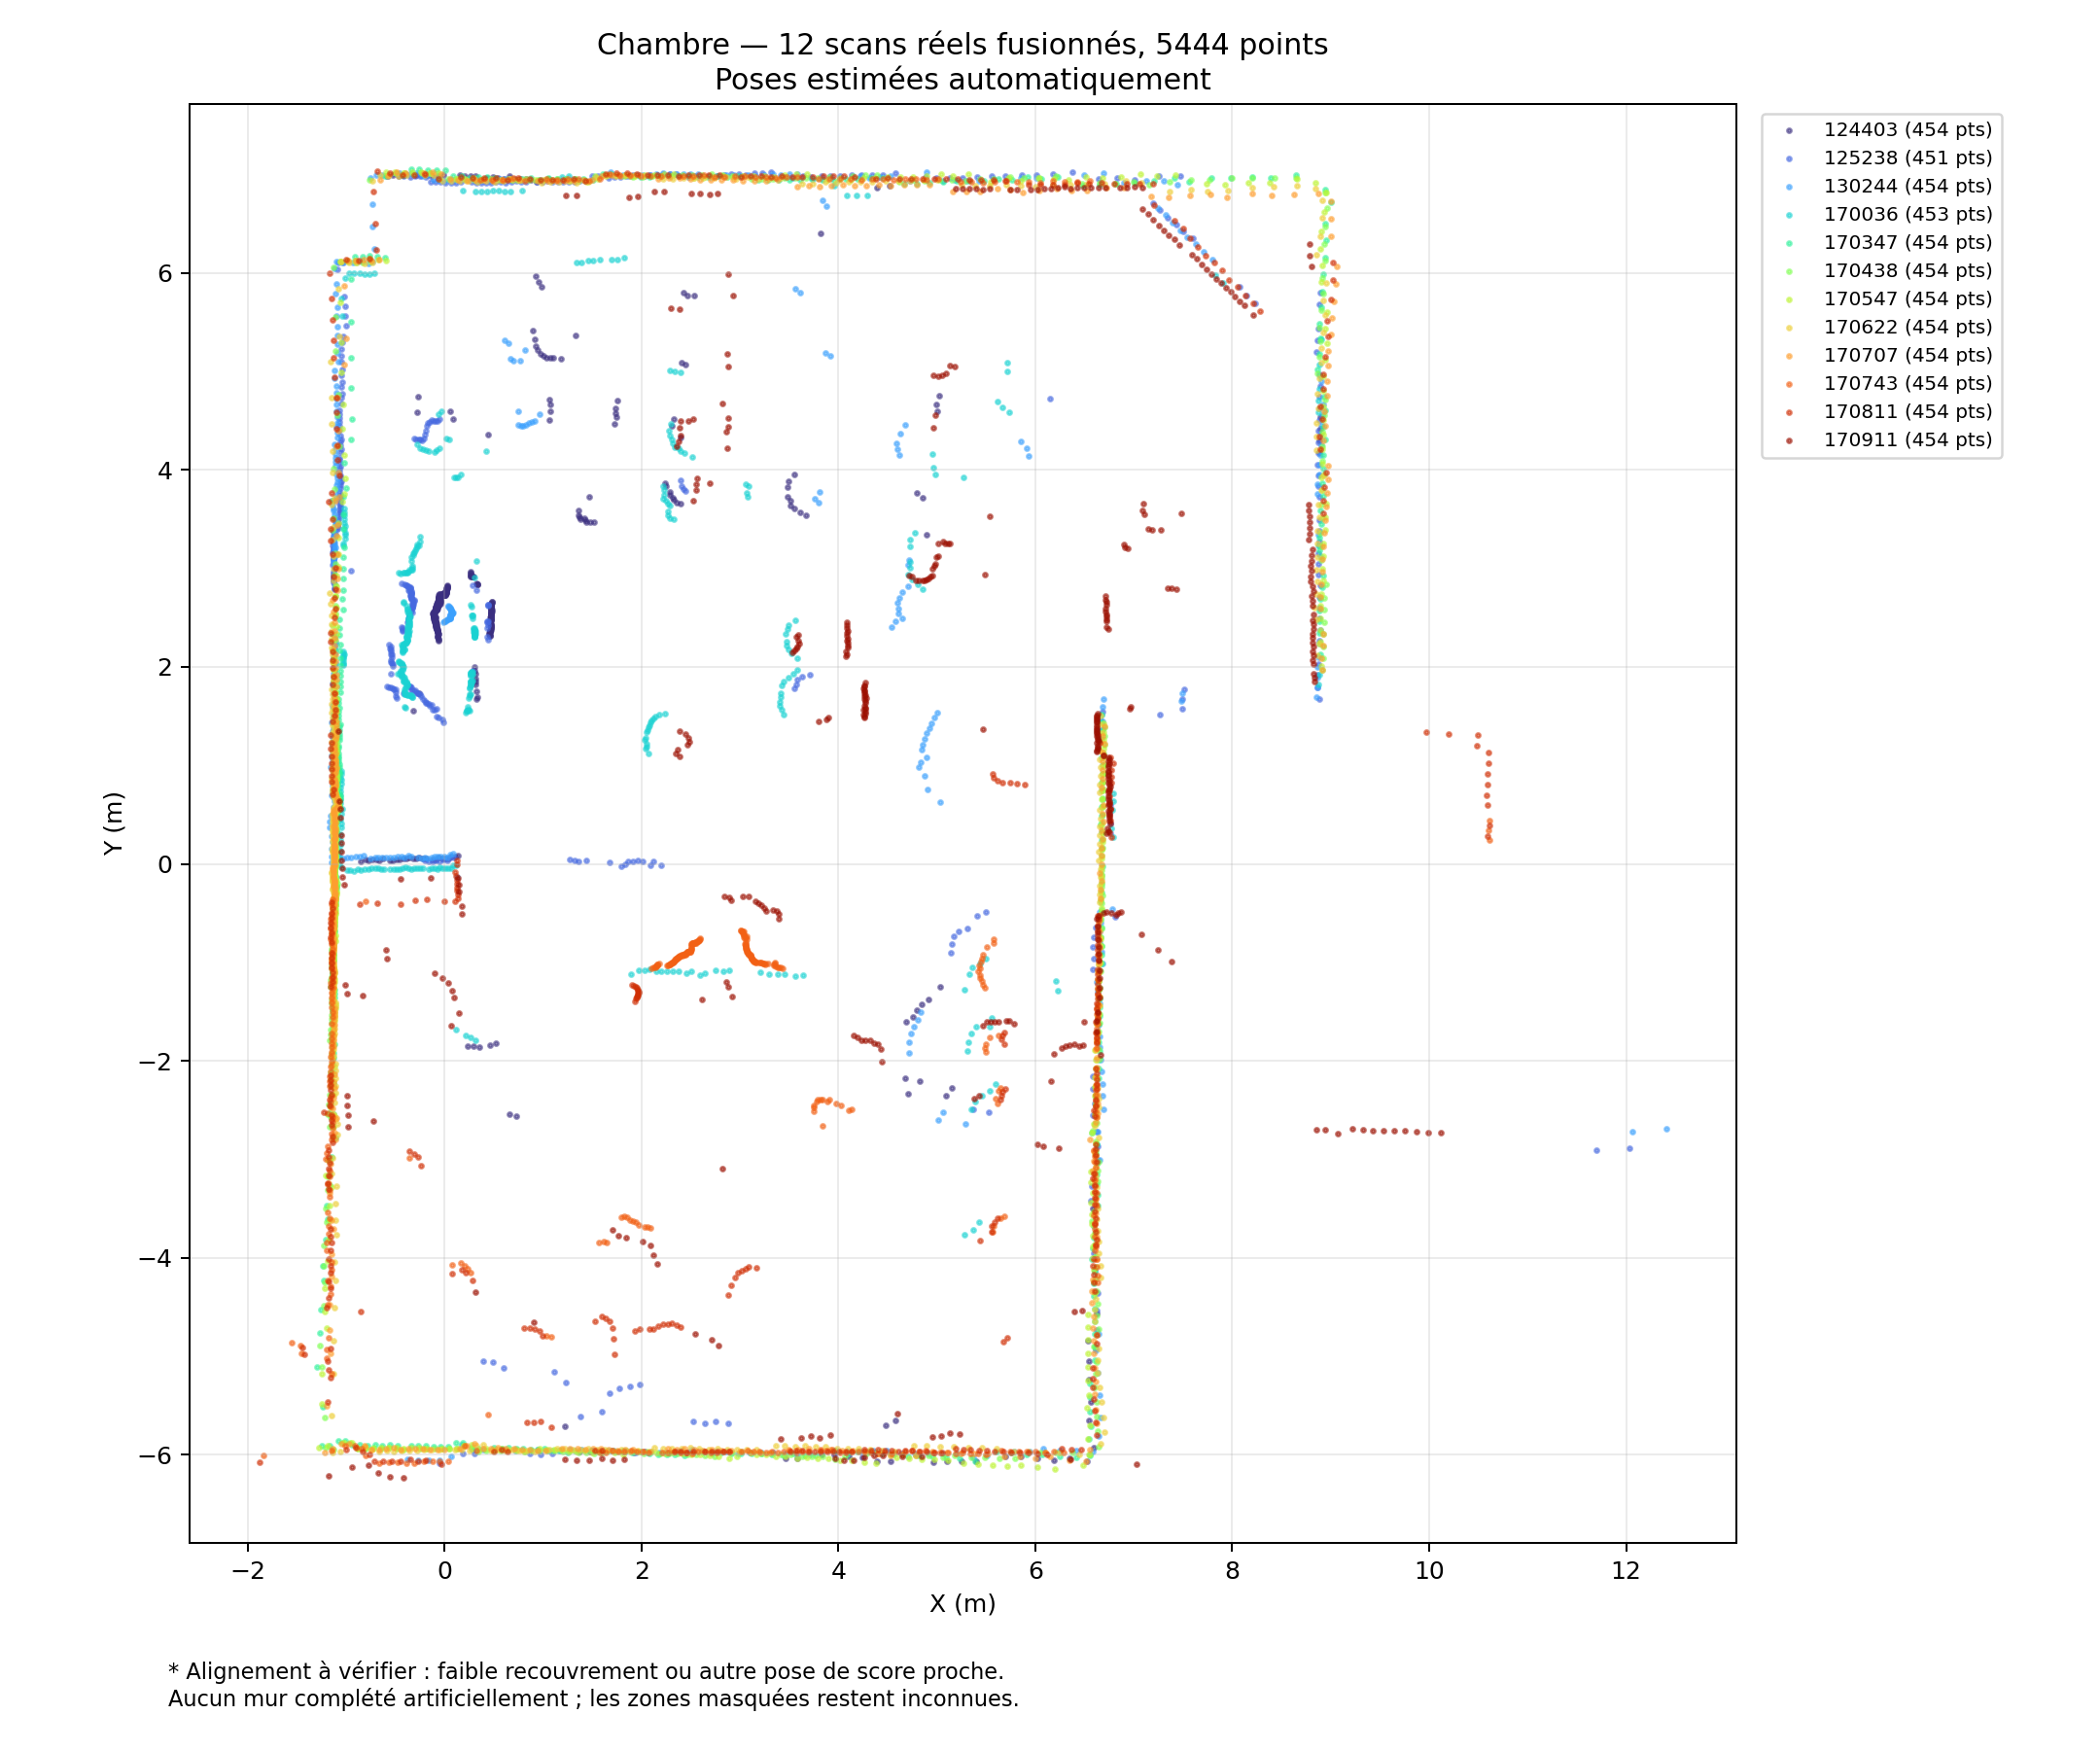
\includegraphics[width=0.73\linewidth]{chambre_fusionnee.png}
\caption{Nuage fusionné des acquisitions réelles. Les surfaces intérieures
peuvent correspondre aux objets présents dans la salle. L'alignement reste estimé.}
\end{figure}

\clearpage
\section{Construction d'une carte d'occupation 2D}
\subsection{Principe et mise à jour}
La grille utilise des cellules carrées de \textbf{5 cm de côté}. Chaque
cellule représente un espace libre, occupé, ou encore inconnu/incertain.
Pour une origine métrique $(o_x,o_y)$ et une résolution $r$, les indices sont
obtenus par discrétisation :
\[
 c=\left\lfloor\frac{x-o_x}{r}\right\rfloor,\qquad
 l=\left\lfloor\frac{y-o_y}{r}\right\rfloor.
\]
L'origine de la grille est alignée sur les cellules. La grille s'agrandit
si une nouvelle acquisition dépasse les limites déjà représentées, sans
perdre les observations antérieures.

Pour chaque mesure valide, l'algorithme de Bresenham parcourt les cellules
entre la pose du LiDAR et l'impact. Les cellules traversées reçoivent une
observation libre ; la dernière reçoit une observation occupée. Les cellules
derrière l'impact et celles situées entre les rayons ne deviennent pas libres
sans observation. Si une cellule est à la fois traversée et touchée par un
impact dans le même scan, l'impact est prioritaire.

\subsection{Accumulation probabiliste}
Les observations sont accumulées en log-odds :
\[
 L(c)=\log\!\left(\frac{p(c)}{1-p(c)}\right),\qquad
 L_{t+1}(c)=\operatorname{clip}\bigl(L_t(c)+\Delta L,\,-4,\,4\bigr).
\]
Les incréments choisis sont $-0{,}40$ pour une observation libre et
$+0{,}85$ pour une observation occupée. Une cellule est mise à jour au plus
une fois par scan, afin que plusieurs rayons du même scan ne surpondèrent
pas artificiellement son état.

Les seuils sont $p\leq0{,}45$ pour libre et $p\geq0{,}65$ pour occupé.
Les probabilités intermédiaires et les cellules jamais observées sont
représentées en gris. Le masque des cellules observées est conservé.

\subsection{Implémentation et résultats}
Dans \code{gridmap.py}, \code{scan_to_map} construit une carte à partir
d'un scan et de sa pose ; \code{update_map} met à jour une carte existante.
Les exports comprennent une image PNG, une matrice CSV, les métadonnées
JSON et un fichier NPZ conservant les observations pour une mise à jour.
Dans le CSV, $-1$ signifie inconnu/incertain, $0$ libre et $1$ occupé.
La première ligne correspond au $Y$ minimal.

\begin{table}[htbp]
\centering
\caption{Résultats des cartes d'occupation, à une résolution de 5 cm.}
\begin{tabular}{lrrrr}
\toprule
Carte & Impacts & Colonnes $\times$ lignes & Cellules libres & Occupées \\
\midrule
Scan 1 & 454 & $277\times268$ & 24\,050 & 384 \\
Scan 2 & 454 & $269\times210$ & 28\,330 & 381 \\
Scan 3 & 454 & $207\times268$ & 28\,191 & 381 \\
Fusion & 5\,444 & $291\times271$ & 46\,065 & 1\,110 \\
\bottomrule
\end{tabular}
\end{table}

\subsubsection*{Version améliorée : tracé des rayons vectorisé}
Dans la version d'origine, \code{update_map} parcourait les rayons un par
un en Python. La nouvelle fonction \code{trace_rays} exécute le même
algorithme de Bresenham sur \emph{tous les rayons à la fois} : la boucle
porte sur la longueur du plus long rayon, et chaque pas applique aux
vecteurs NumPy la même arithmétique entière (erreur cumulée, pas en $x$
et en $y$). Les cellules traversées et les cellules d'impact sont donc
strictement les mêmes ; la règle selon laquelle un impact du même scan
n'est pas effacé par un autre rayon est conservée.

\begin{itemize}
\item \textbf{Équivalence} : un test compare 60 mises à jour aléatoires
(dont des impacts dans la cellule du robot) à l'implémentation d'origine ;
les log-odds et les cellules observées sont identiques bit à bit. Les quatre
cartes du tableau ci-dessus sont régénérées à l'identique.
\item \textbf{Temps} : sur Scan 1 (454 impacts), une mise à jour passe de
34 ms à 13 ms, soit un facteur 3 environ. Le gain reste modéré car les
rayons d'une pièce sont courts (2 à 4 m, soit 40 à 80 cellules) ; il compte
surtout au TP n° 3, où la carte est mise à jour à chaque scan et
reconstruite après chaque fermeture de boucle.
\end{itemize}

Plusieurs impacts peuvent atteindre la même cellule ; le nombre de cellules
occupées n'est donc pas égal au nombre de mesures. Les cartes individuelles
utilisent chacune la pose conventionnelle $(0,0,0^\circ)$ dans leur propre
repère et ne doivent pas être directement superposées. La carte Fusion
emploie les douze poses estimées.

\clearpage
\begin{figure}[p]
\centering
\begin{subfigure}{0.48\linewidth}
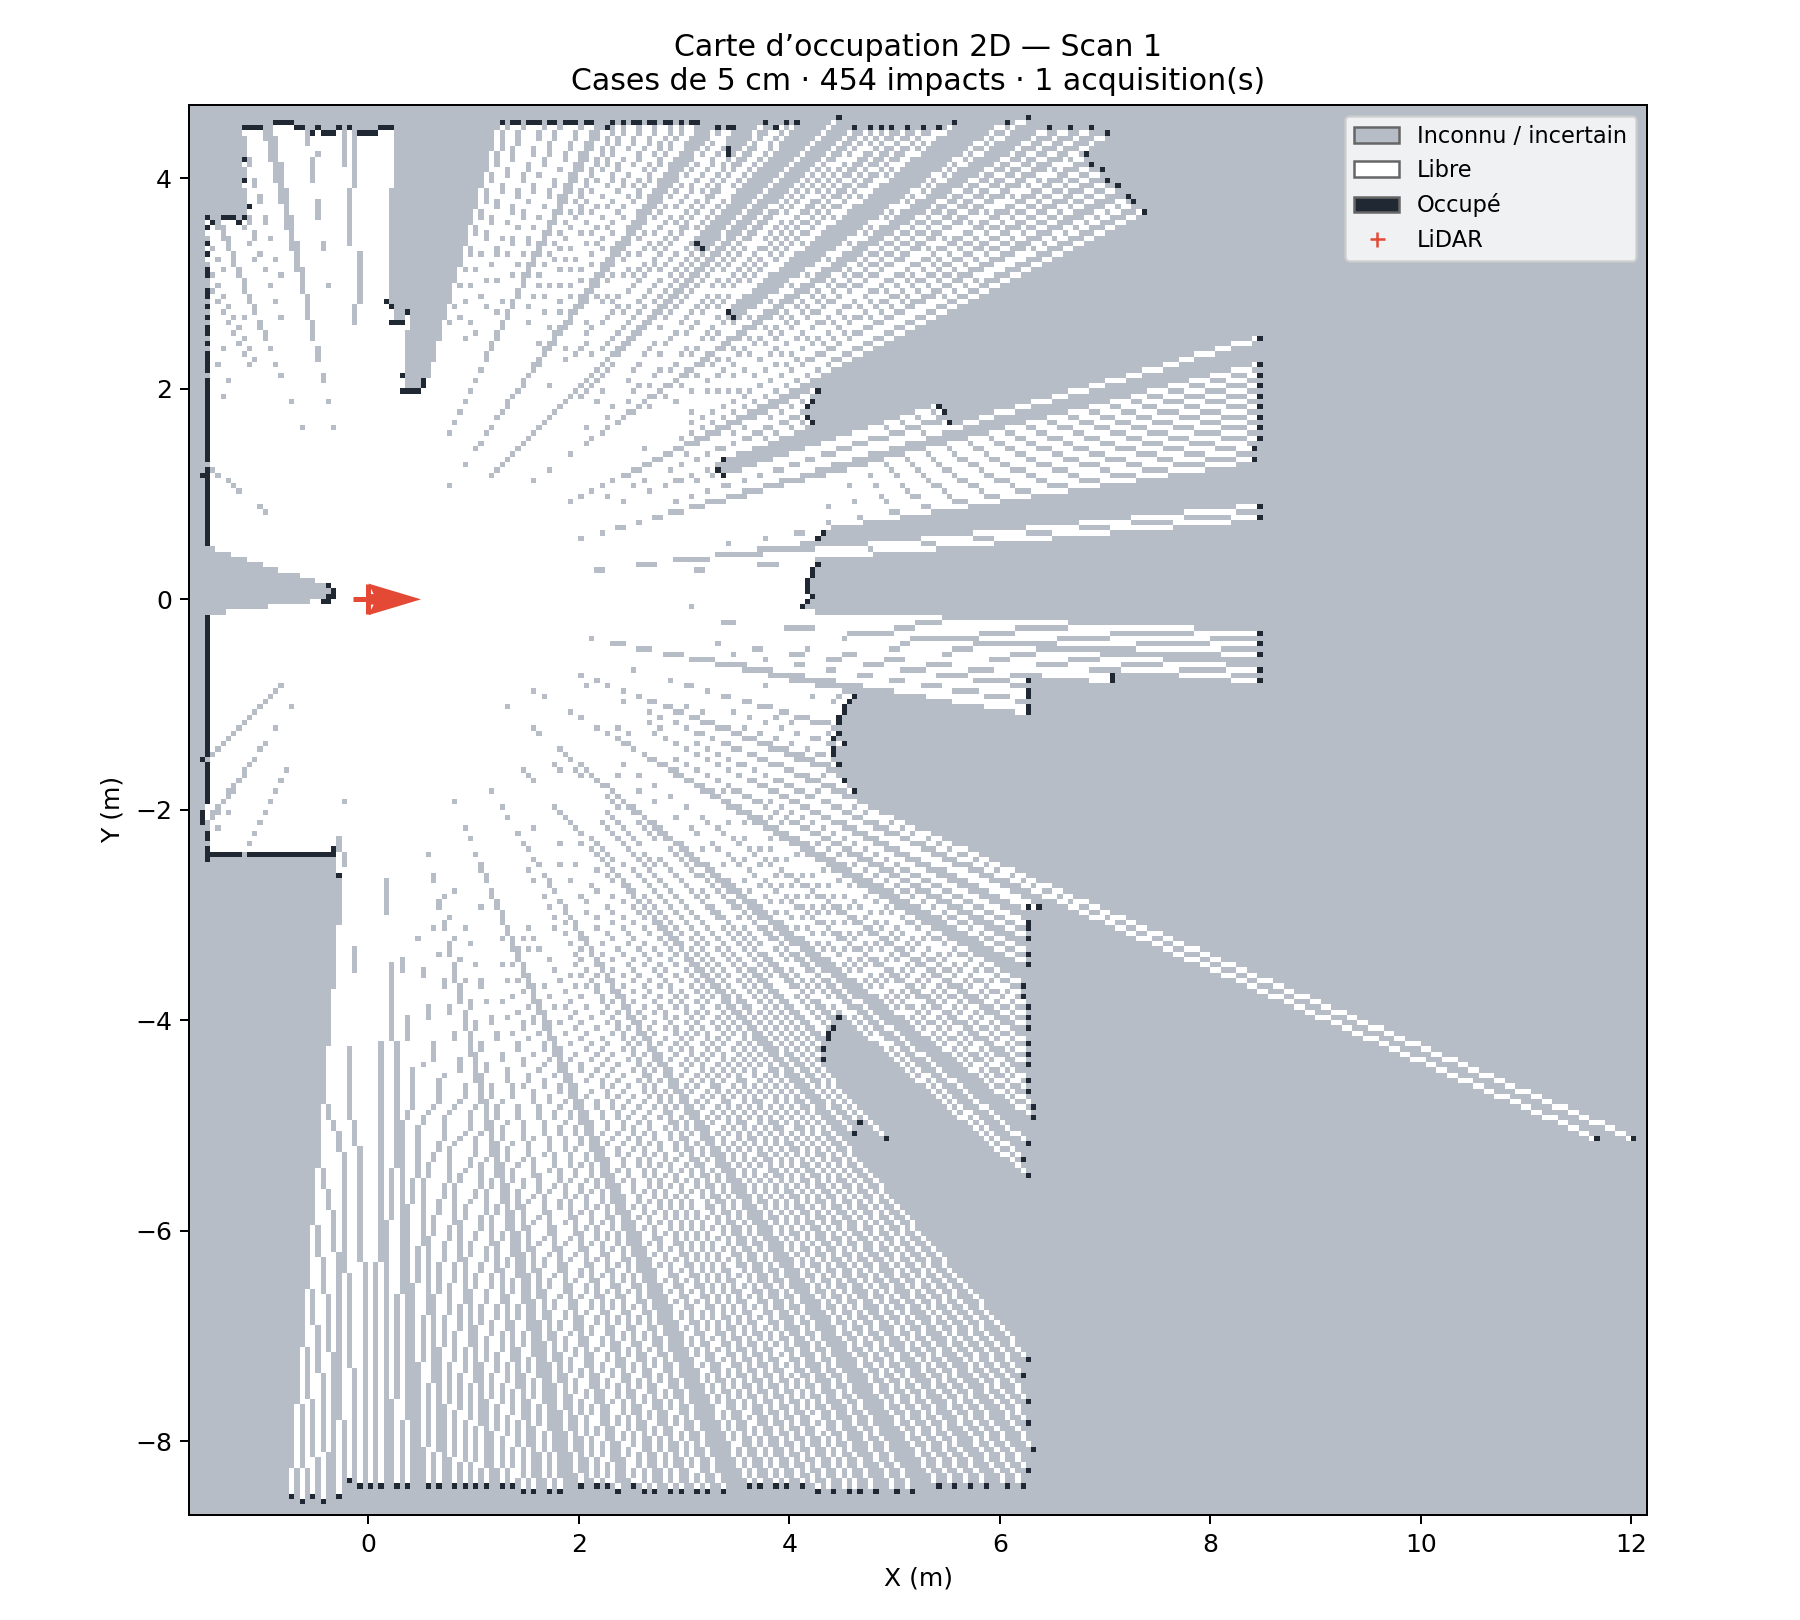
\includegraphics[width=\linewidth]{carte_occupation_2d_scan_1.png}
\caption{Scan 1}
\end{subfigure}\hfill
\begin{subfigure}{0.48\linewidth}
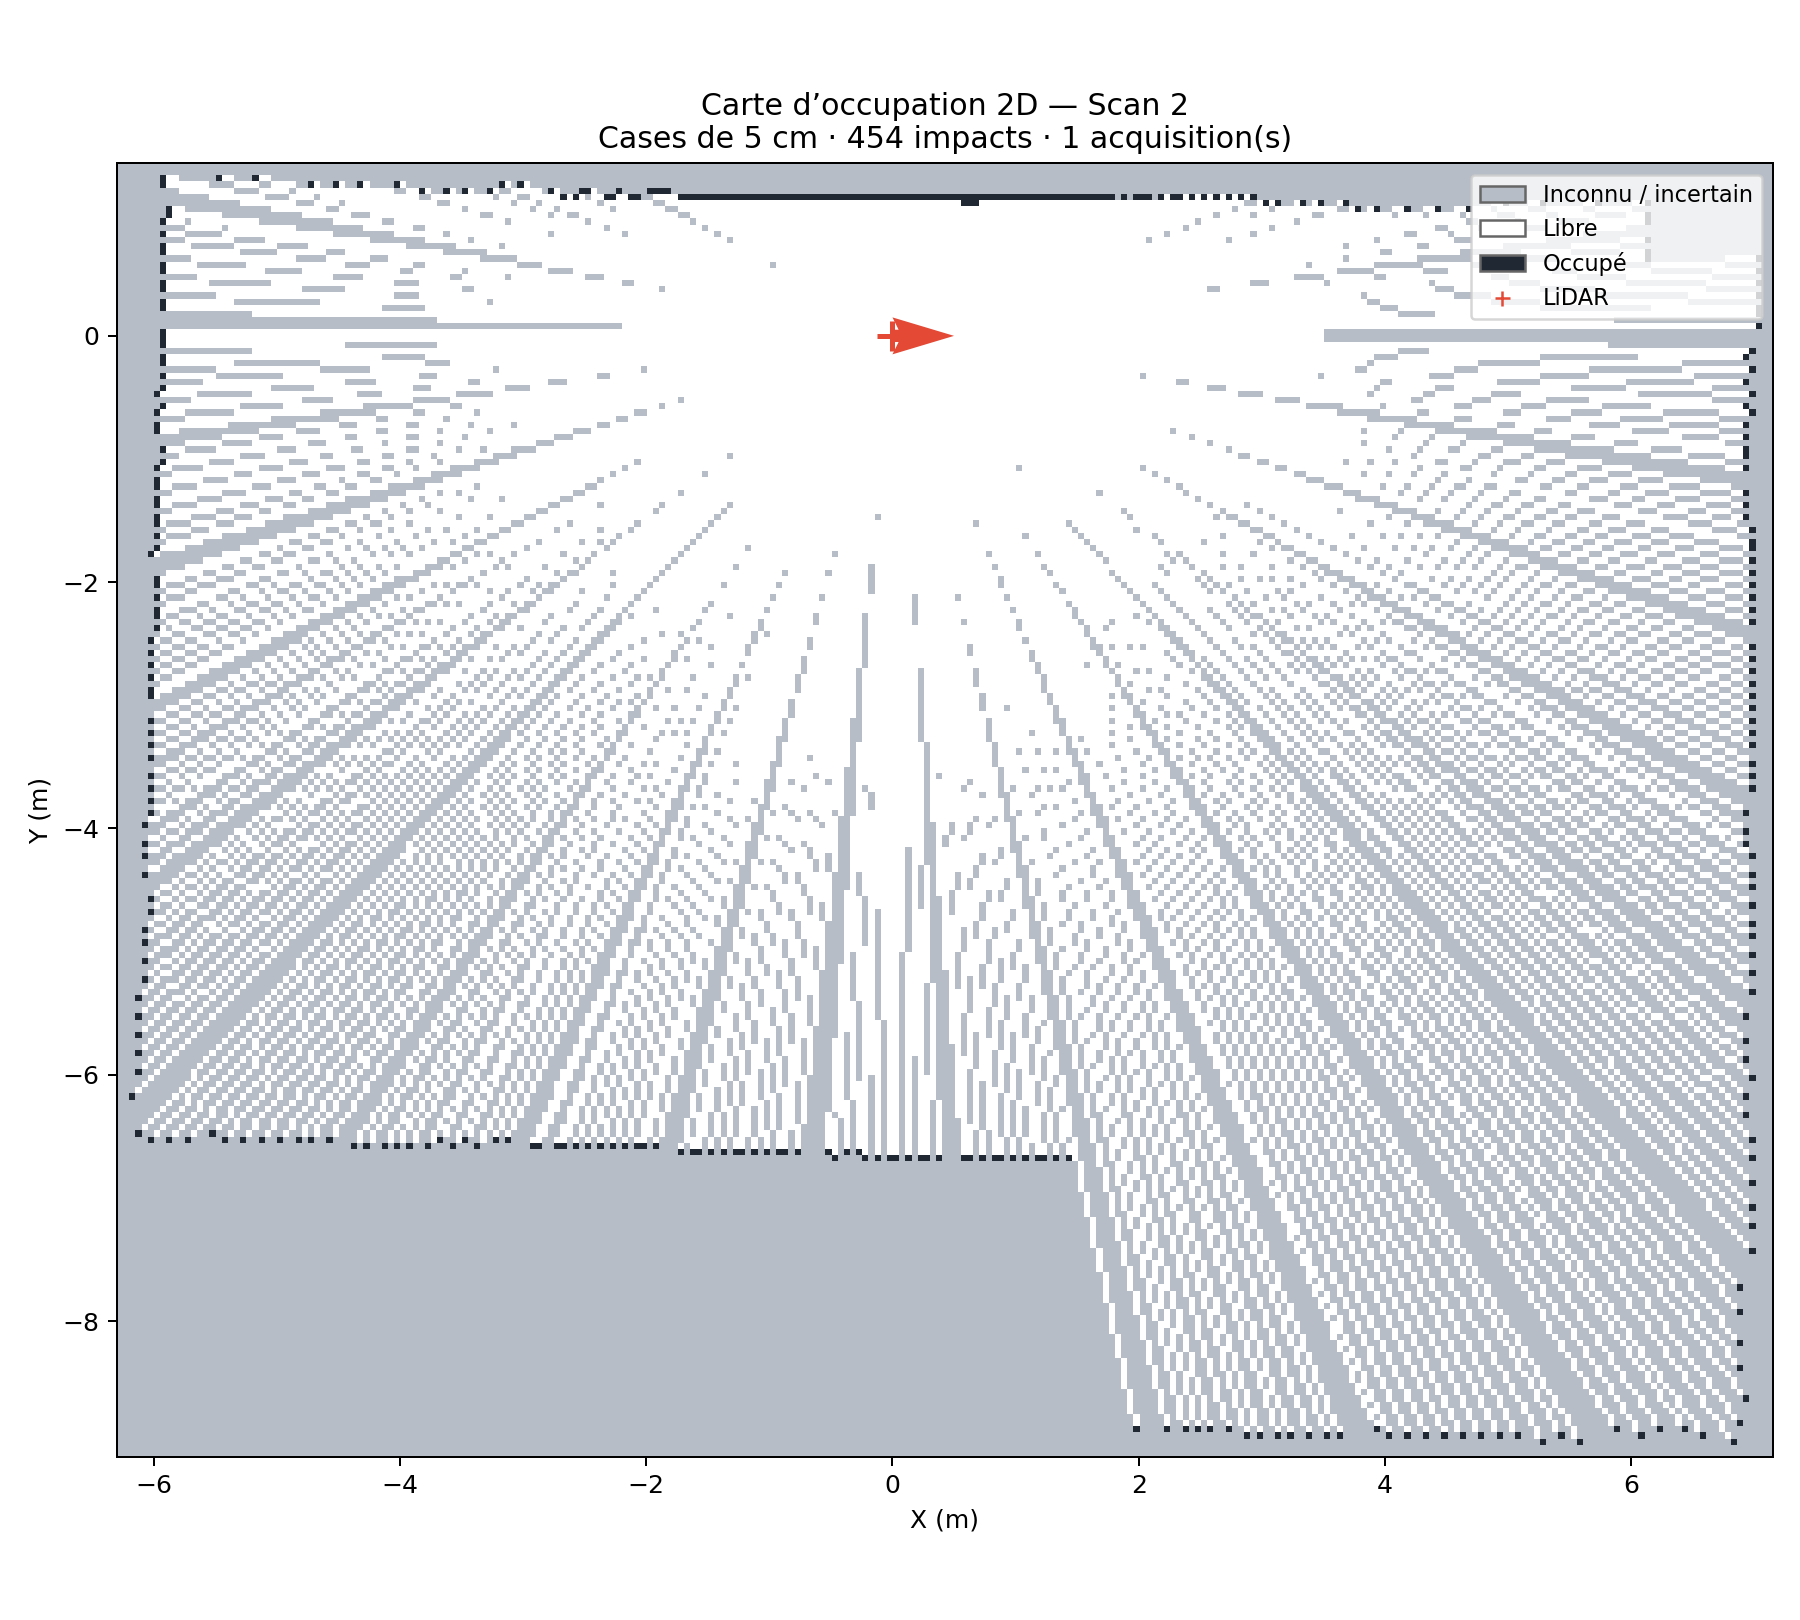
\includegraphics[width=\linewidth]{carte_occupation_2d_scan_2.png}
\caption{Scan 2}
\end{subfigure}
\par\medskip
\begin{subfigure}{0.48\linewidth}
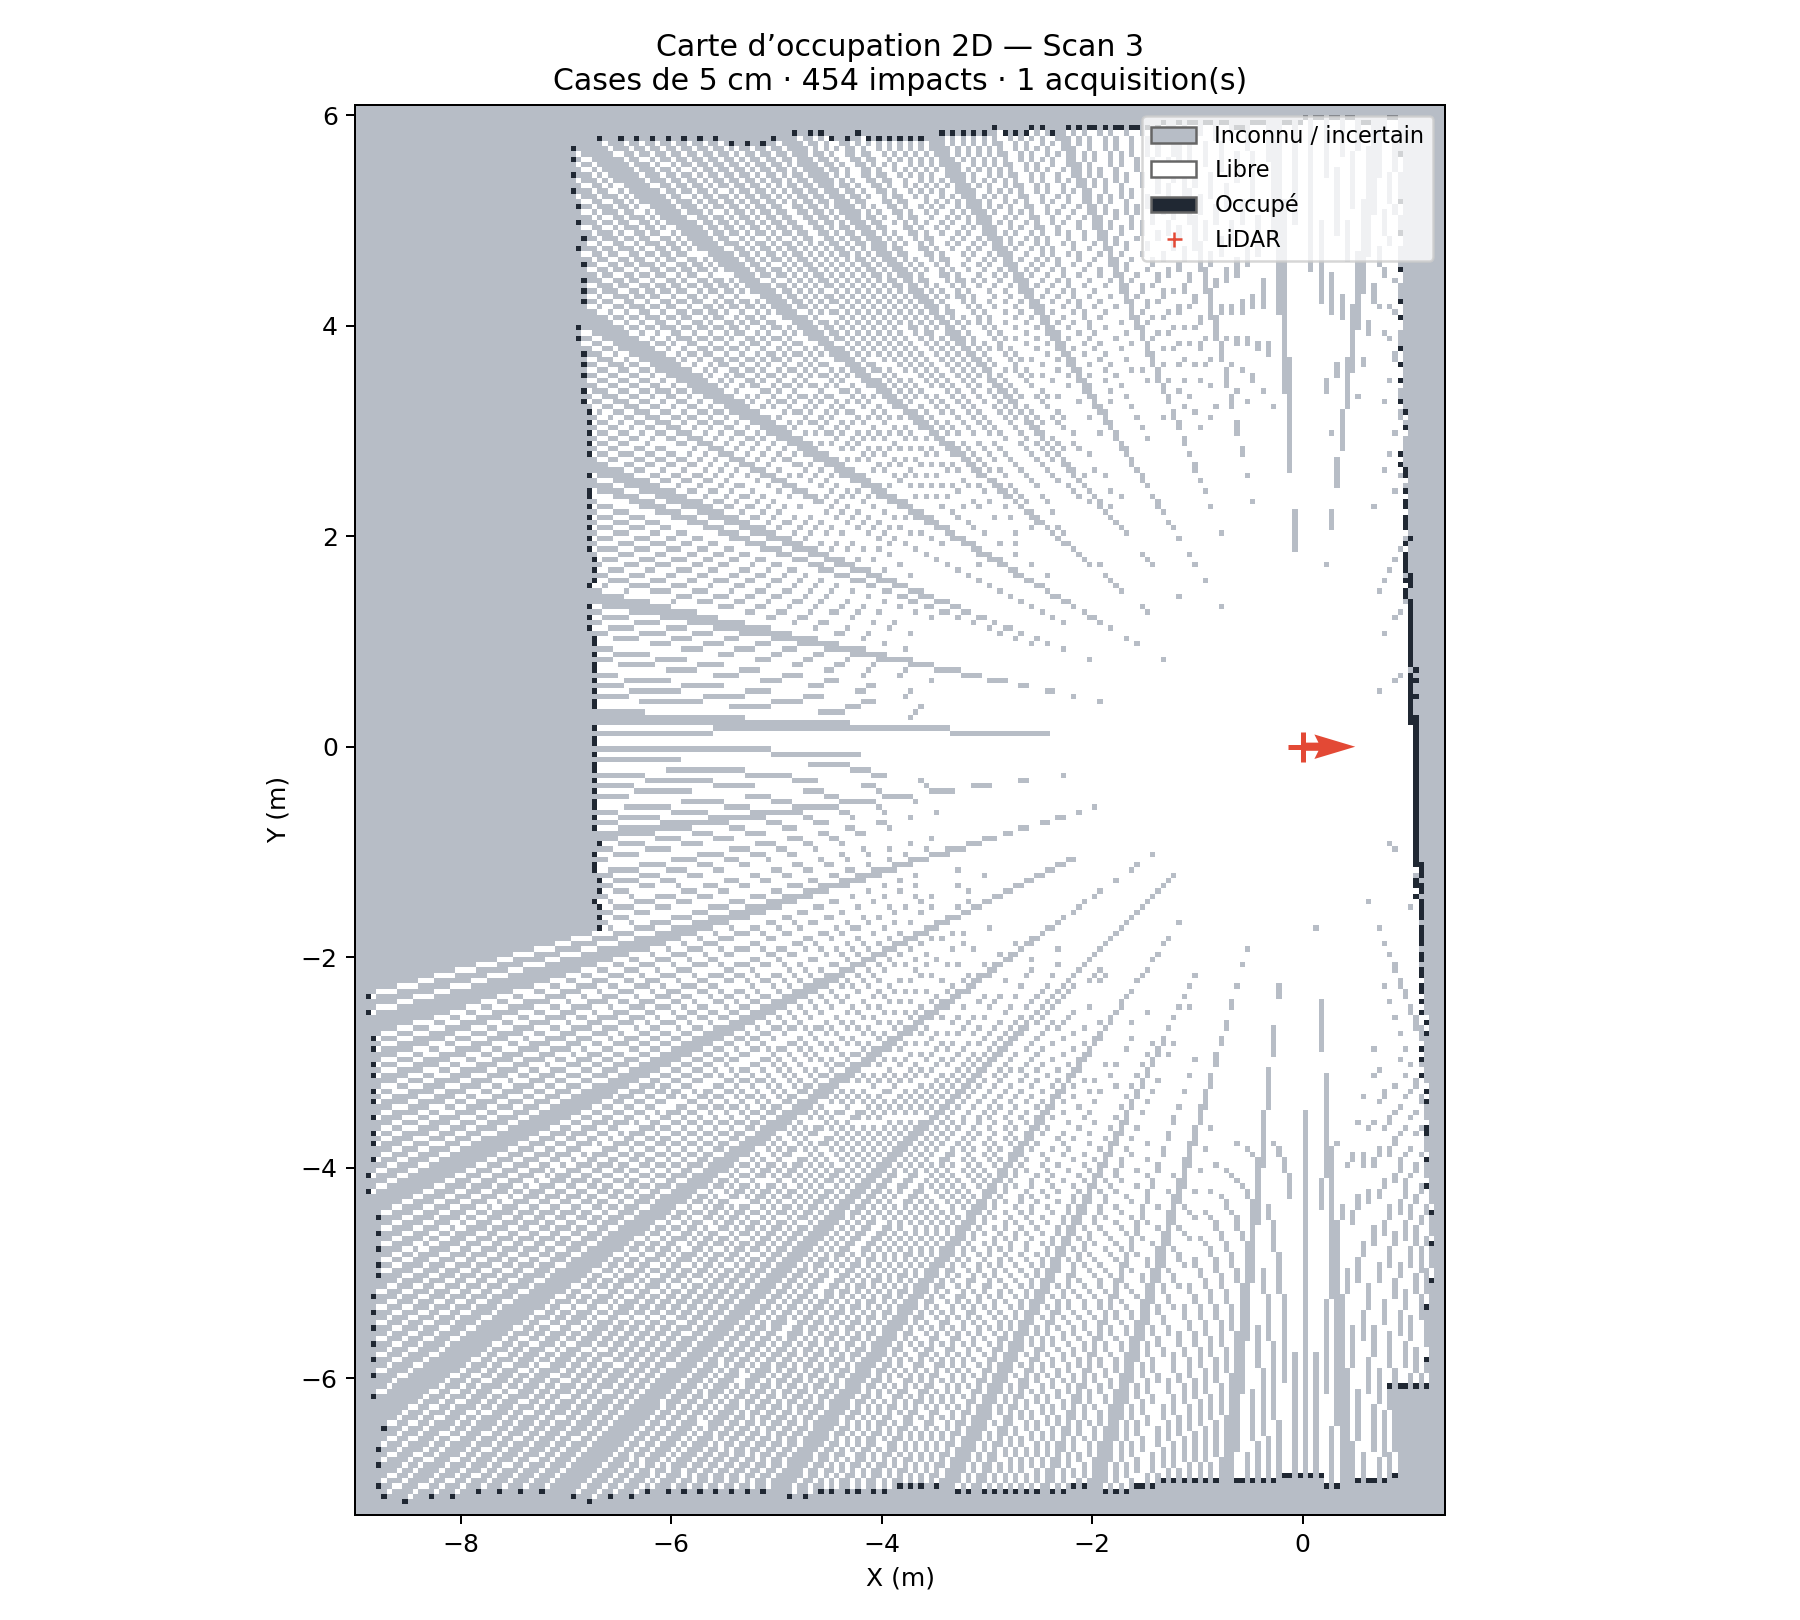
\includegraphics[width=\linewidth]{carte_occupation_2d_scan_3.png}
\caption{Scan 3}
\end{subfigure}\hfill
\begin{subfigure}{0.48\linewidth}
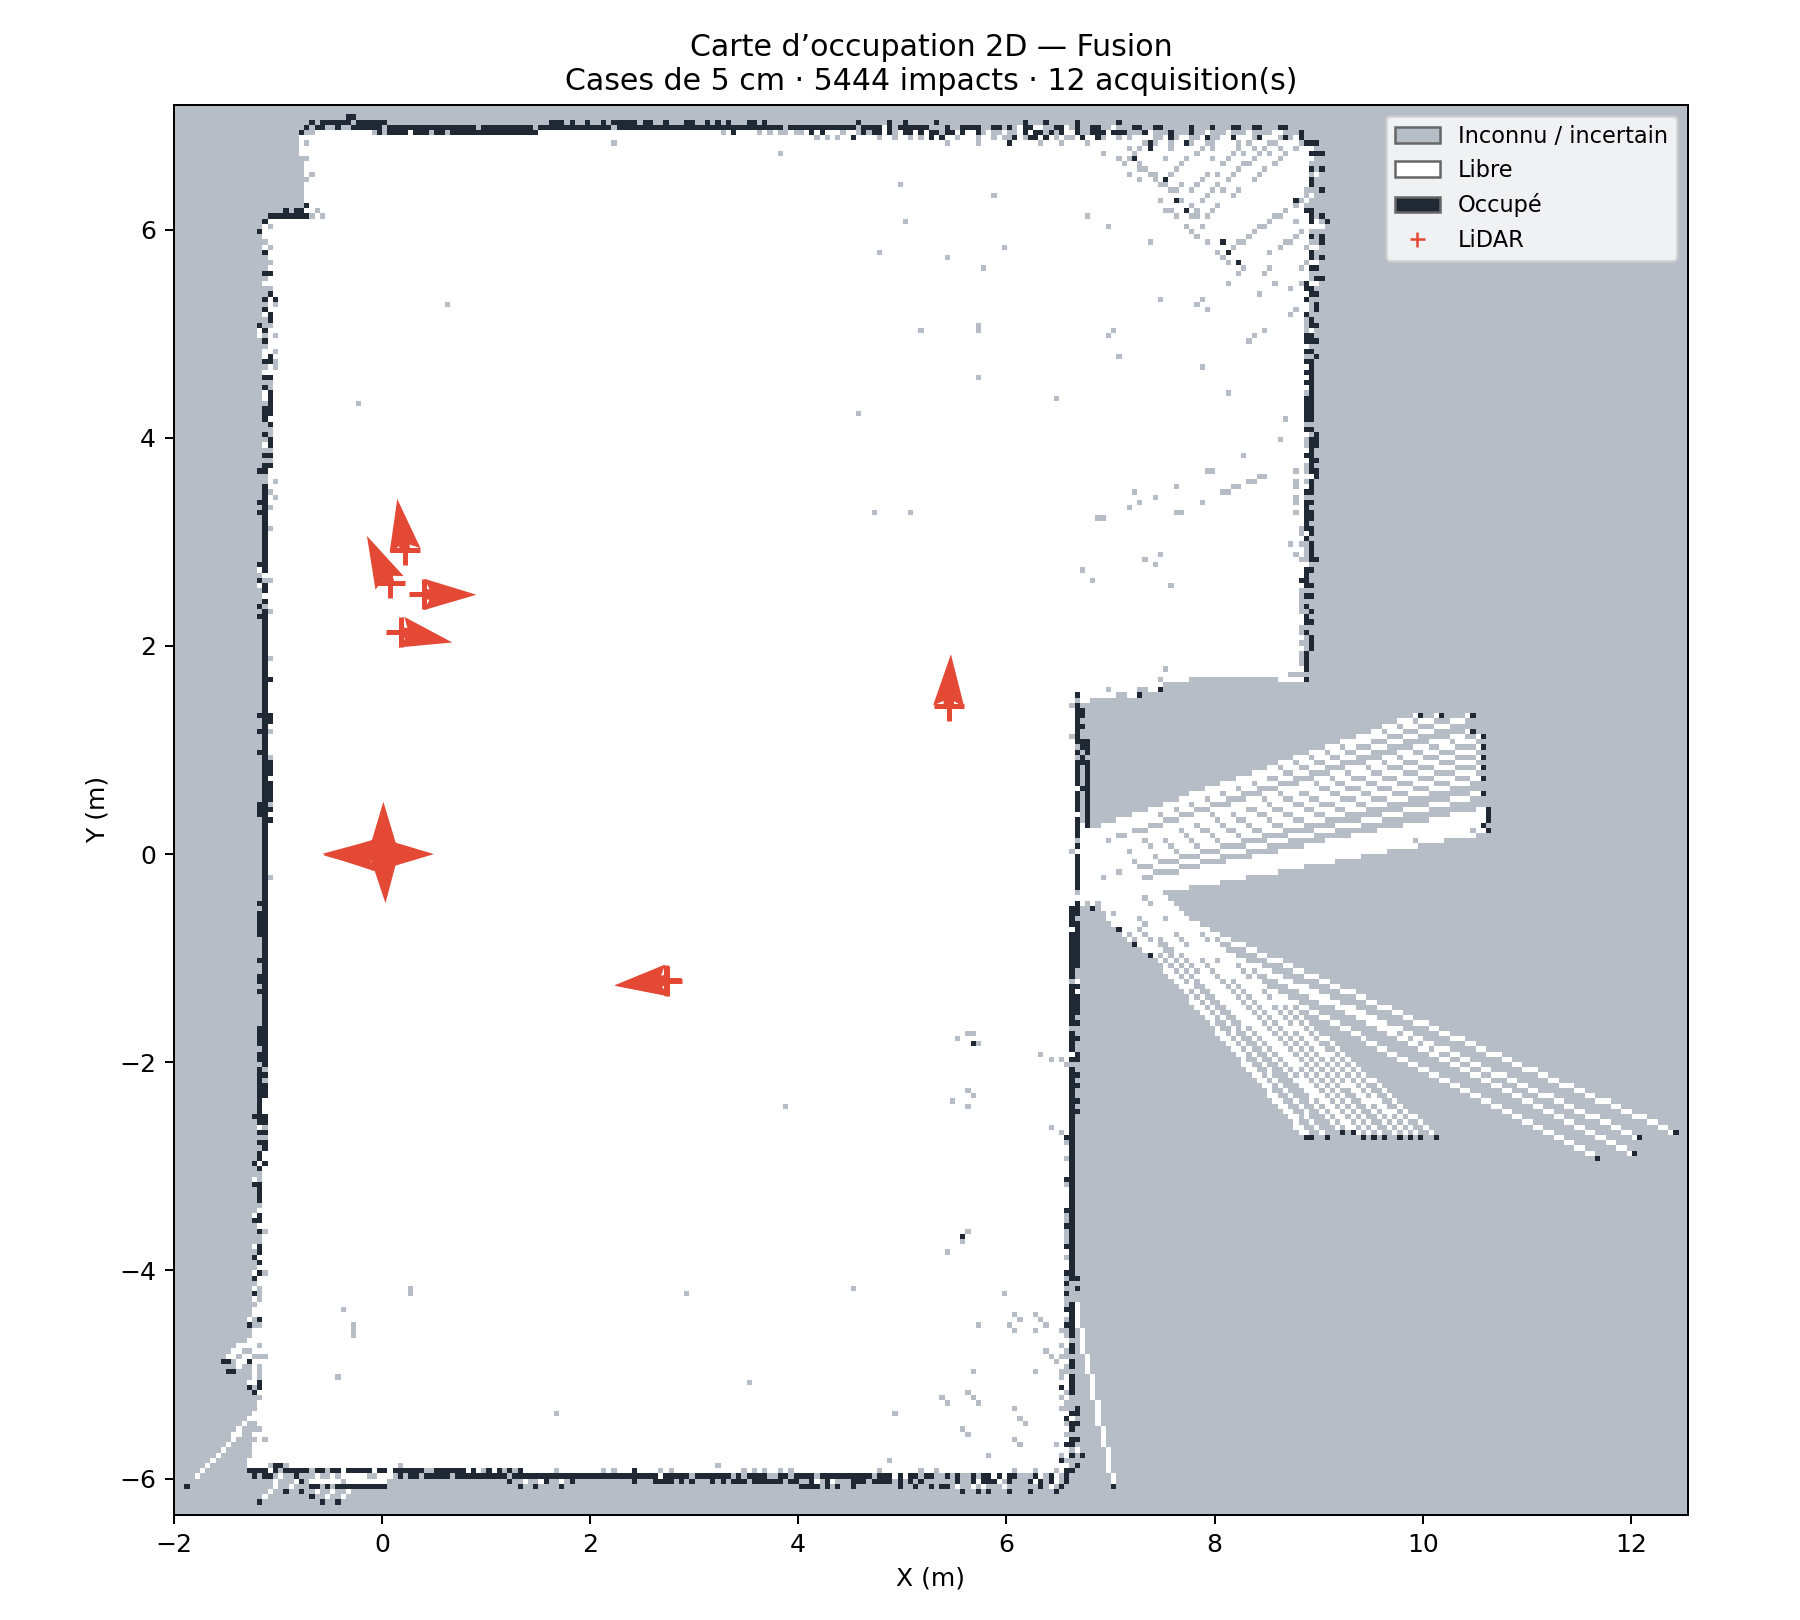
\includegraphics[width=\linewidth]{carte_occupation_2d_fusion.png}
\caption{Fusion des douze acquisitions}
\end{subfigure}
\caption{Cartes d'occupation : blanc = libre, noir = occupé,
gris = inconnu ou incertain. Les origines LiDAR sont en rouge.
Chaque graphique conserve sa propre échelle et son propre cadrage.}
\end{figure}
\clearpage
\section{Extraction et manipulation de segments}
\subsection{Extraction par subdivision et fusion}
Le module \code{segments.py} transforme les points d'un scan en segments
candidats avec une méthode de type \emph{split-and-merge} :
\begin{enumerate}[nosep]
\item Trier les points selon leur angle autour de l'origine du scan.
\item Ouvrir le parcours circulaire à sa plus grande rupture, puis séparer
les groupes lorsque deux points consécutifs sont éloignés de plus de 50 cm.
\item Ajuster une droite par analyse en composantes principales (ACP).
\item Subdiviser si l'écart perpendiculaire maximal dépasse 5 cm.
\item Réunir les groupes voisins si leur différence d'angle ne dépasse pas
$10^\circ$ et si tous les points respectent encore le seuil de 5 cm.
\end{enumerate}
Un segment retenu doit avoir au moins six points de support et une longueur
de 25 cm. Une rupture initiale interdit de fusionner les groupes de part et
d'autre pendant cette extraction. Les extrémités sont les projections
extrêmes des points sur la droite ajustée. Ces seuils sont des paramètres
choisis pour les données disponibles, et non des propriétés connues de la salle.

\subsection{Opérations géométriques}
L'angle entre deux segments est non orienté :
\[
 \alpha=\arccos\!\left(
 \frac{|\mathbf u\cdot\mathbf v|}{\|\mathbf u\|\,\|\mathbf v\|}
 \right)\in[0,\pi/2].
\]
Il ne dépend pas du sens choisi pour les extrémités. La proximité combine
un critère angulaire et la distance entre les segments finis ; deux
segments parallèles mais éloignés ne sont donc pas considérés comme proches.
La fusion ajuste une droite ACP aux extrémités des segments compatibles.

Pour l'intersection, les équations paramétriques sont
$A+t\mathbf u=B+s\mathbf v$. Une intersection n'est acceptée que si elle
appartient aux deux segments, compte tenu de la tolérance numérique.
Les cas parallèles et colinéaires n'ont pas d'intersection ponctuelle
utilisable pour le découpage.

\subsection{Règle de découpage et cas limites}
La tolérance métrique est fixée à $\varepsilon=10^{-6}$ m. Une intersection
doit être strictement intérieure au segment à couper ; un contact à une
extrémité ne change rien. Le plus long des deux côtés est conservé.
Si leurs longueurs sont égales à la tolérance près, le côté contenant le
premier point du segment est retenu.

Les tests couvrent les croisements en X, les deux choix de côté, l'égalité
exacte et à $\pm10^{-8}$ m, les contacts en extrémité, un contact à
l'extrémité du coupeur, les segments colinéaires et parallèles, et les
intersections situées en dehors des segments.

\begin{figure}[htbp]
\centering
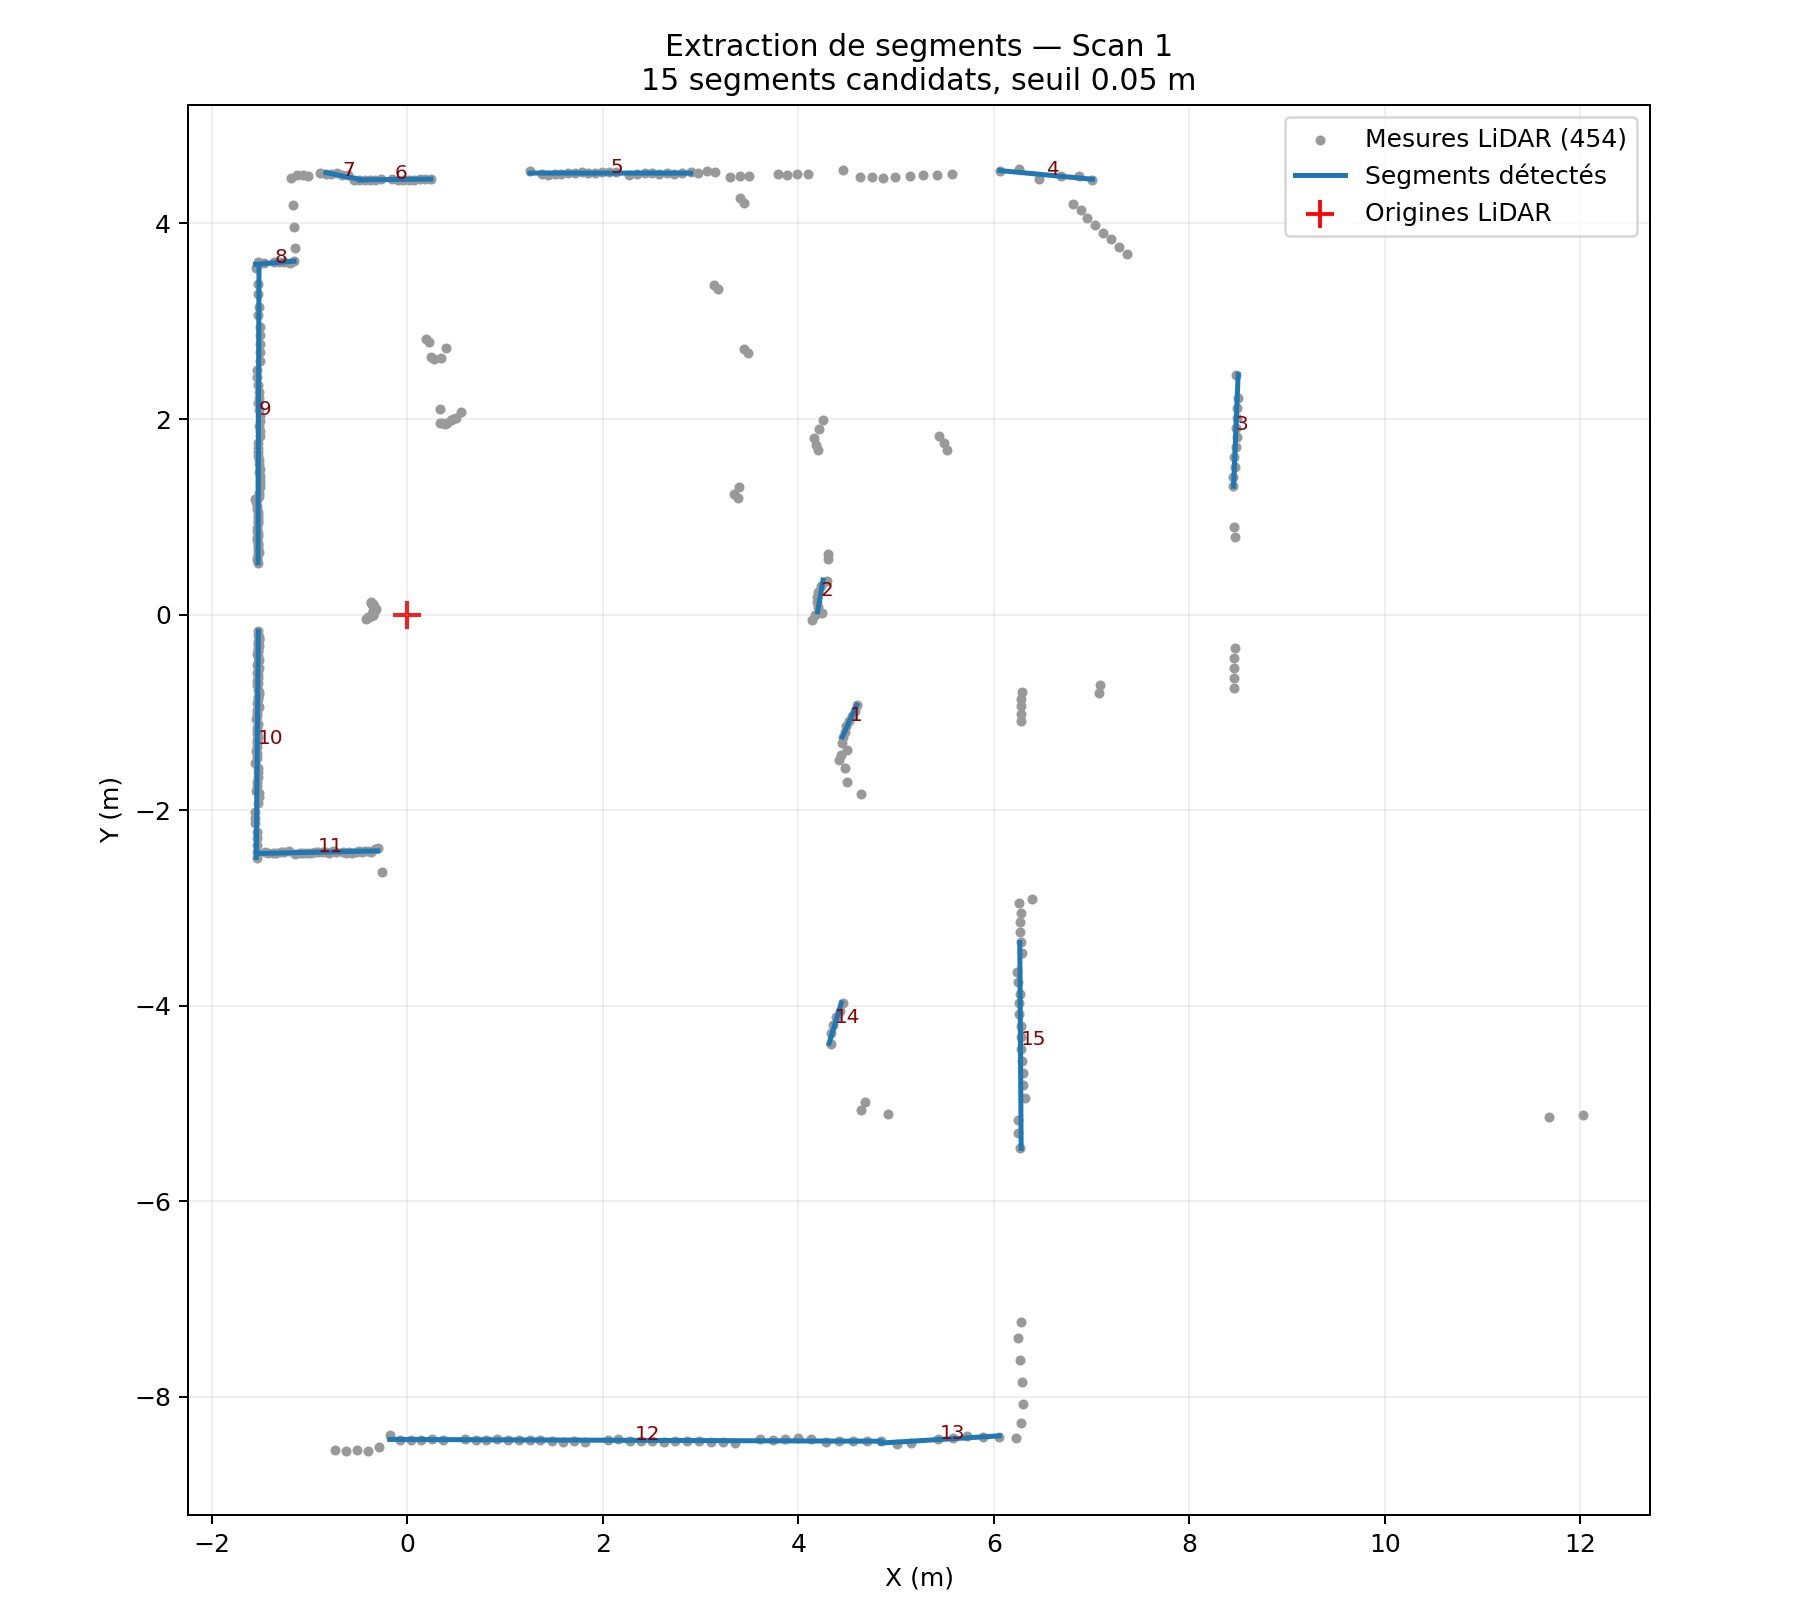
\includegraphics[width=0.68\linewidth]{segments_scan_1.png}
\caption{Scan 1 : 15 segments extraits des 454 impacts valides.
Les points isolés ou groupes trop courts ne sont pas transformés en segments.}
\end{figure}

\clearpage
\section{Construction de la carte vectorielle}
\subsection{Association et consolidation}
Le module distinct \code{vectormap.py} réutilise les fonctions de l'étape
précédente. Les segments sont extraits dans chaque repère local, puis placés
dans le repère commun. La consolidation recherche ensuite des segments
compatibles, y compris entre acquisitions différentes.

La fusion d'une paire exige simultanément :
\begin{itemize}
\item une différence d'angle inférieure ou égale à $8^\circ$ ;
\item une distance entre les segments finis inférieure ou égale à 20 cm ;
\item un écart de chaque extrémité à la droite de l'autre segment
inférieur ou égal à 8 cm ;
\item un écart maximal de tous les supports à la nouvelle droite ACP
inférieur ou égal à 8 cm.
\end{itemize}
Toutes les extrémités d'origine sont conservées dans les groupes fusionnés,
à poids égal. Cela limite la dérive qui résulterait d'ajustements successifs
utilisant seulement deux extrémités déjà moyennées. Le tri initial est
déterministe, par longueur puis par coordonnées. L'association est gloutonne
et ne garantit pas une solution optimale globale.

Cette consolidation peut relier des lacunes de 20 cm ou moins ; elle ne
reconstitue pas automatiquement les parties masquées et ne force pas une
forme rectangulaire. La méthode \code{VectorMap.update(points, pose)} permet
d'ajouter un scan à une carte en mémoire. La génération des figures traite
tous les segments en une fois ; des mises à jour successives peuvent
aboutir à des regroupements différents.

\subsection{Intersections et découpage}
Les intersections sont affichées en orange et exportées dans le JSON avec
les numéros des segments concernés. Les cartes présentées sont générées
\textbf{sans suppression de branches aux intersections}.

L'option \code{--trim-crossings} applique le découpage au plus long côté
implémenté à l'étape 4. Chaque segment est coupé par les autres segments
d'entrée dans l'ordre de sortie ; les extrémités sont ordonnées
lexicographiquement pour fixer le premier point. Ce mode reste optionnel :
une intersection géométrique ne prouve pas à elle seule qu'une partie
d'obstacle doit être supprimée.

\subsection{Résultats quantitatifs}
\begin{table}[h]
\centering
\caption{Extraction puis consolidation vectorielle.}
\begin{tabular}{lrrr}
\toprule
Carte & Segments extraits & Segments consolidés & Intersections de paires \\
\midrule
Scan 1 & 15 & 15 & 0 \\
Scan 2 & 8 & 7 & 1 \\
Scan 3 & 9 & 9 & 1 \\
Fusion & 156 & 91 & 37 \\
\bottomrule
\end{tabular}
\end{table}

La consolidation de Fusion réduit le nombre de segments de 65, soit environ
41,7\,\%. Cette réduction mesure le regroupement effectué, pas la précision
de la carte. Des doublons restent possibles lorsque les poses estimées
introduisent des décalages supérieurs aux seuils retenus. Les intersections
sont comptées par paire : plusieurs paires peuvent correspondre à un même
voisinage spatial.

\clearpage
\begin{figure}[p]
\centering
\begin{subfigure}{0.48\linewidth}
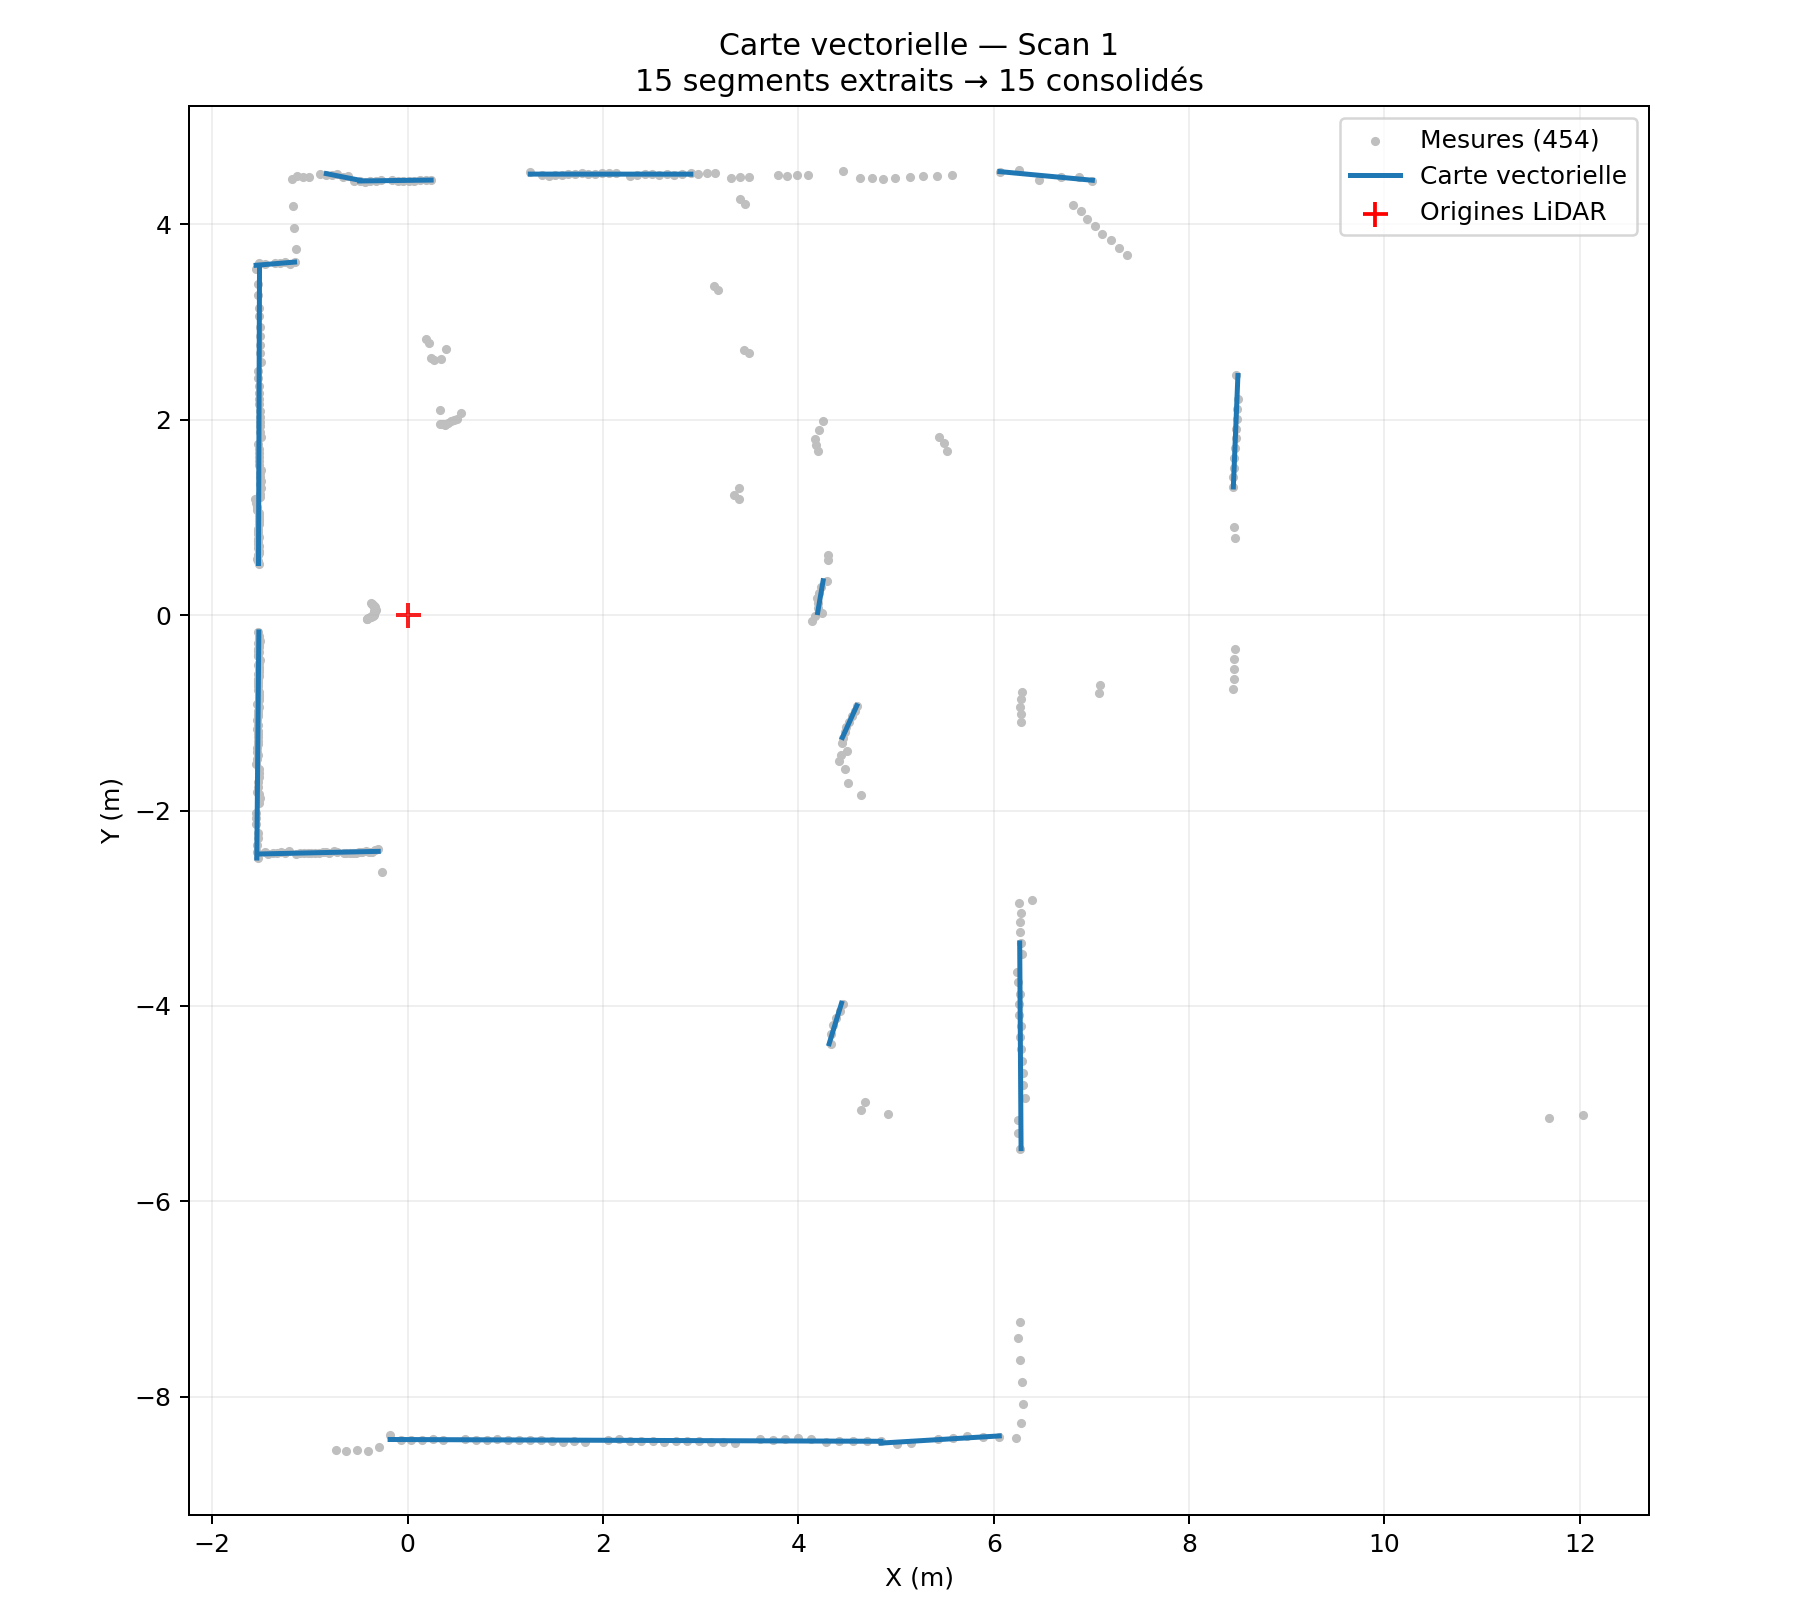
\includegraphics[width=\linewidth]{carte_vectorielle_scan_1.png}
\caption{Scan 1 : 15 segments}
\end{subfigure}\hfill
\begin{subfigure}{0.48\linewidth}
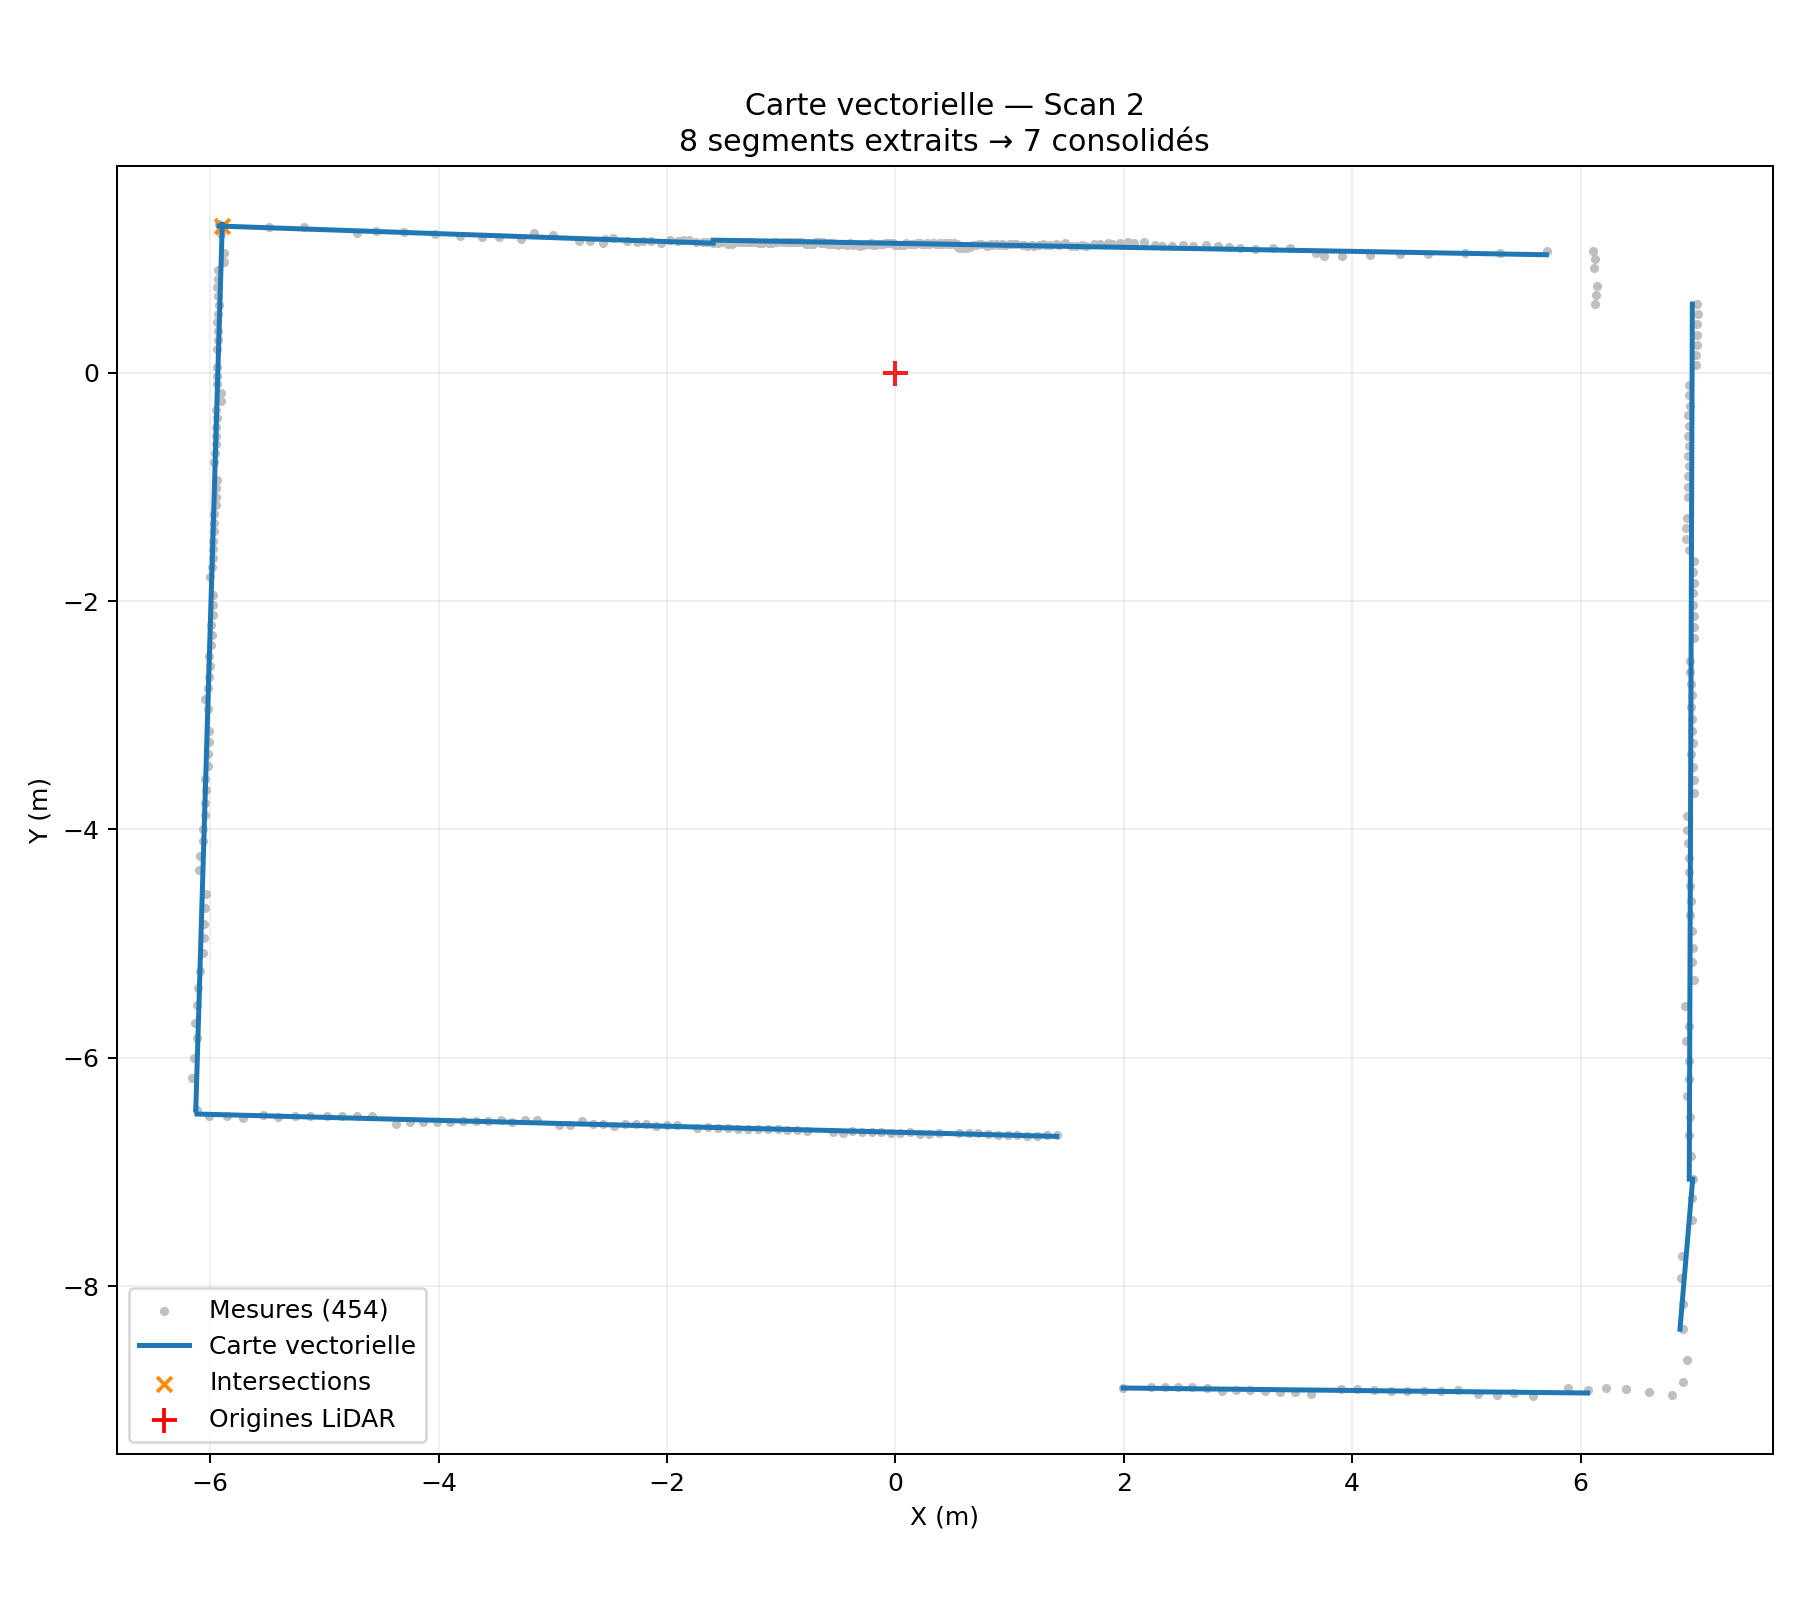
\includegraphics[width=\linewidth]{carte_vectorielle_scan_2.png}
\caption{Scan 2 : 7 segments}
\end{subfigure}
\par\medskip
\begin{subfigure}{0.48\linewidth}
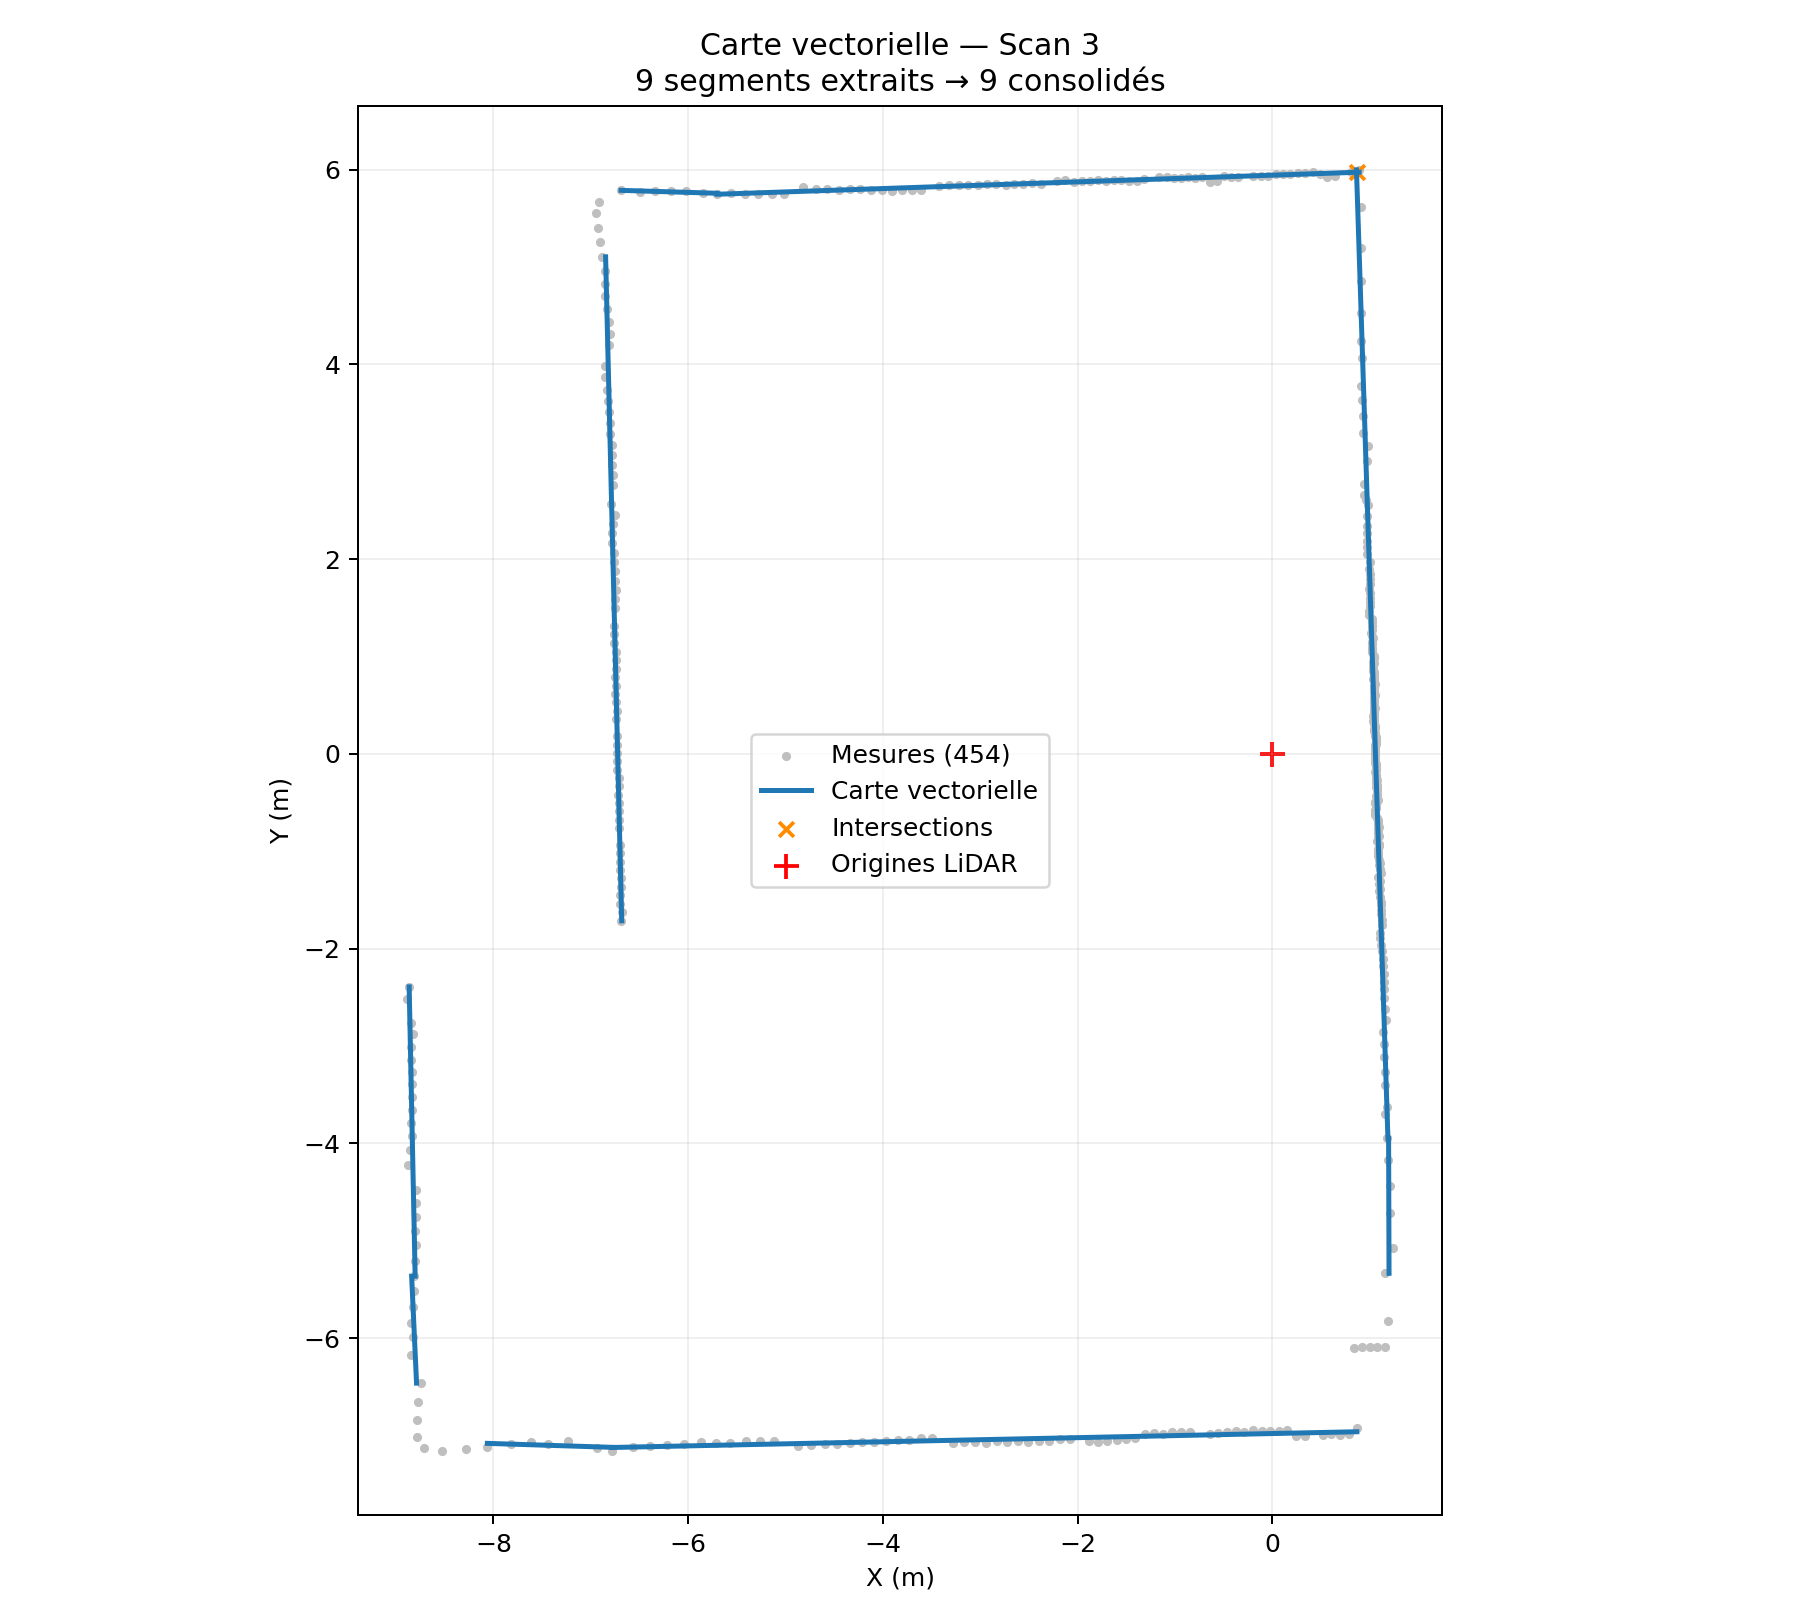
\includegraphics[width=\linewidth]{carte_vectorielle_scan_3.png}
\caption{Scan 3 : 9 segments}
\end{subfigure}\hfill
\begin{subfigure}{0.48\linewidth}
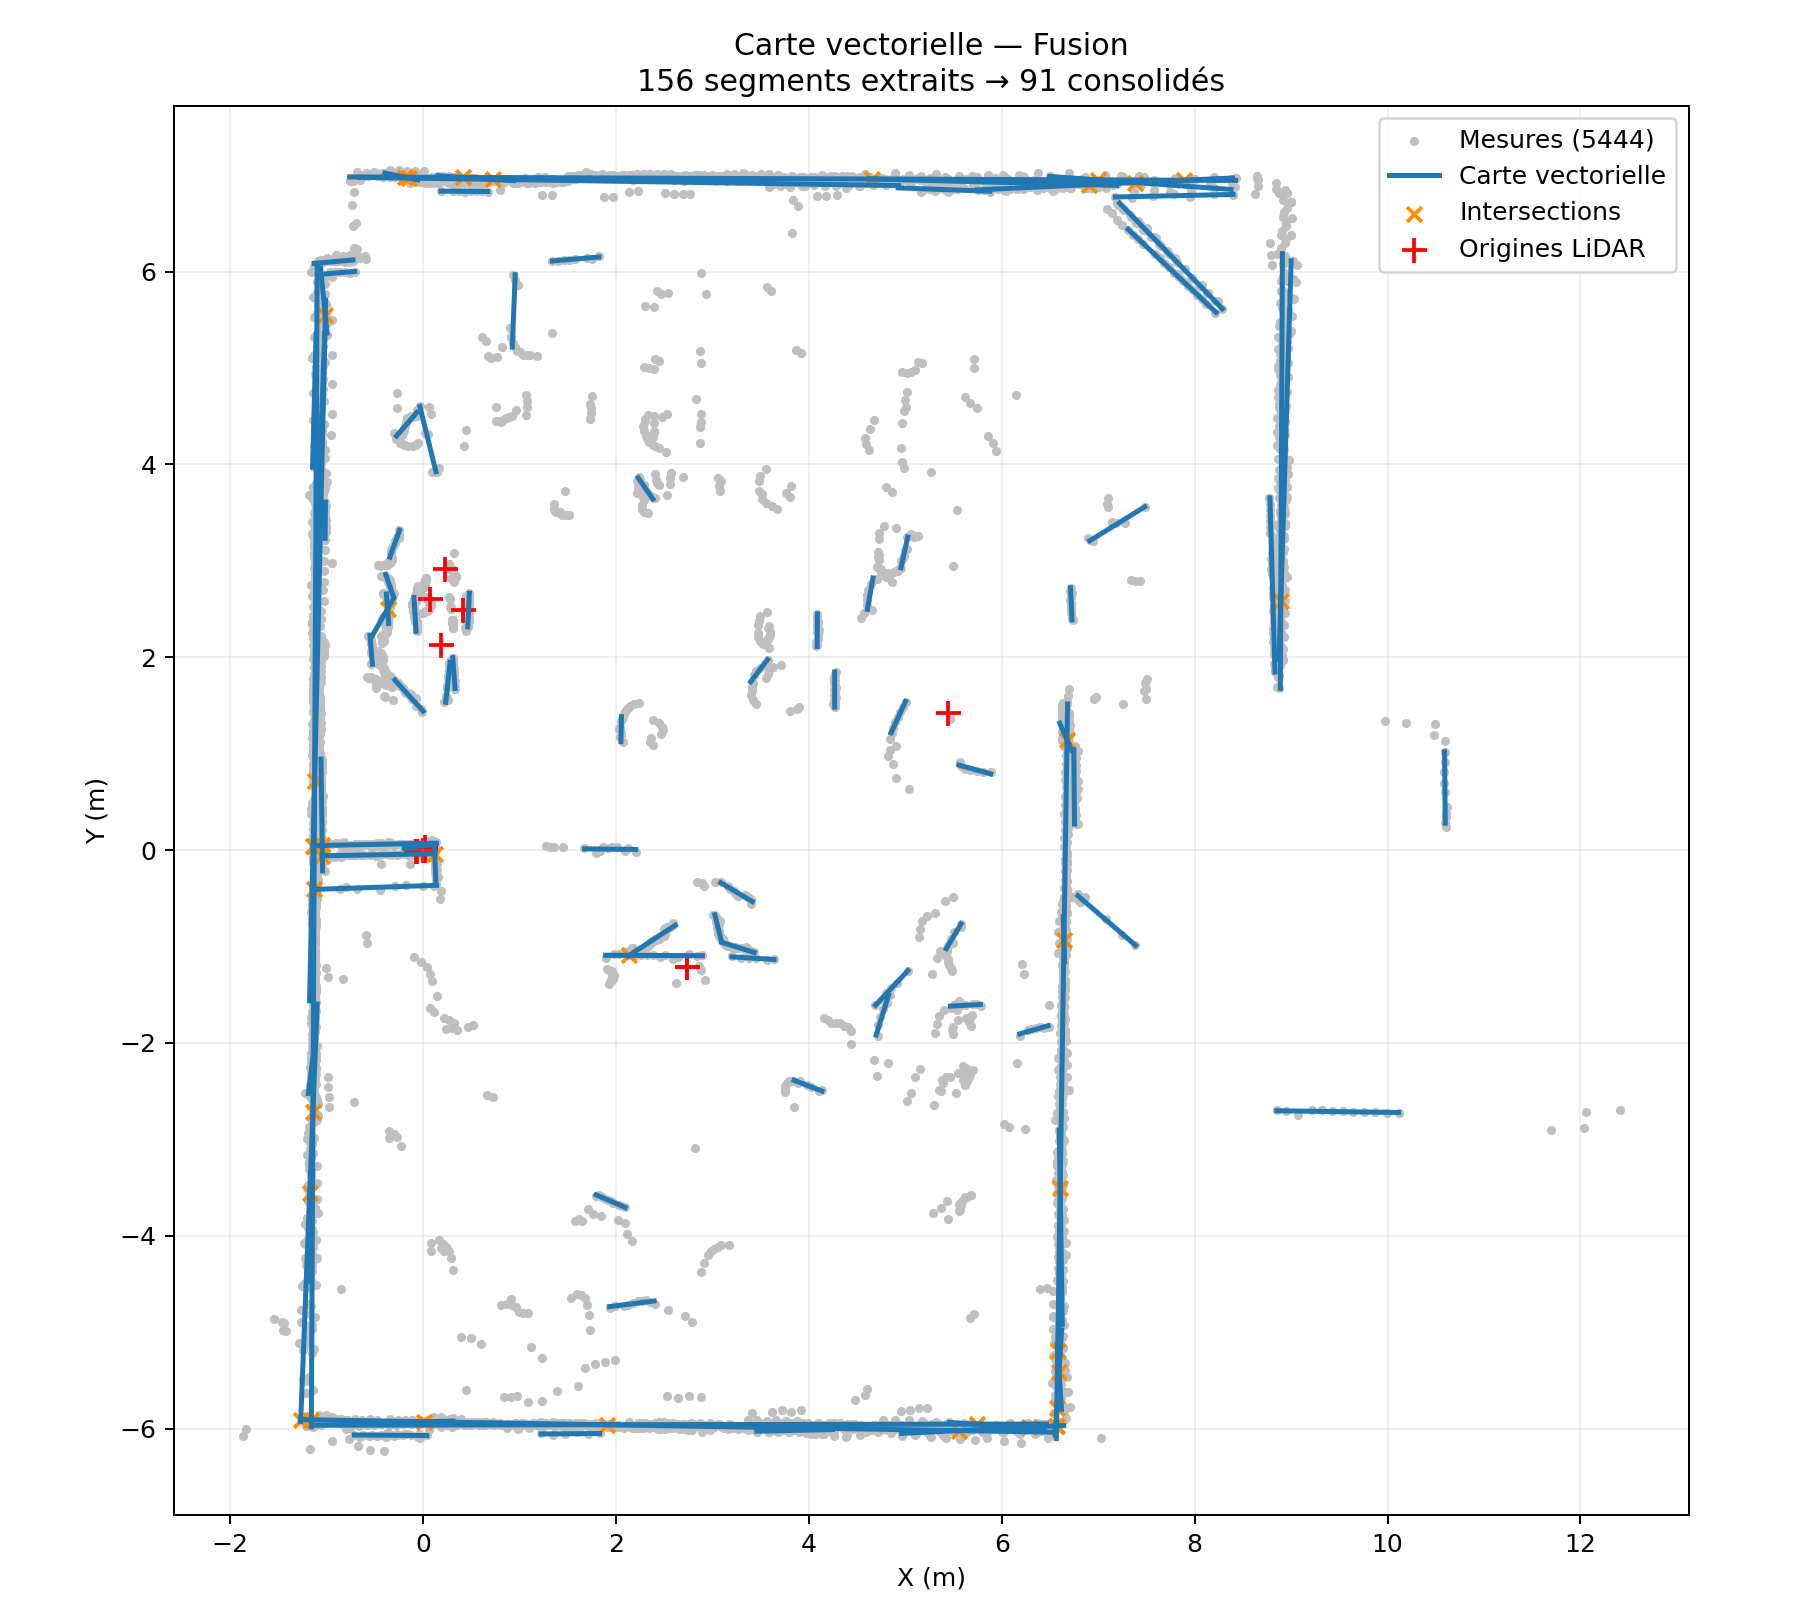
\includegraphics[width=\linewidth]{carte_vectorielle_fusion.png}
\caption{Fusion : 91 segments}
\end{subfigure}
\caption{Cartes vectorielles consolidées, superposées aux mesures.
Les segments décrivent aussi les obstacles intérieurs présents dans la salle.
Les graphiques n'ont pas tous les mêmes limites.}
\end{figure}
\clearpage
\section{Validation et analyse critique}
\subsection{Tests logiciels}
La suite de tests exécutée sur le projet comportait \textbf{48 tests réussis}
pour le TP n° 1. Dans la version améliorée, la suite complète des trois TP
compte \textbf{98 tests réussis}, dont le test d'équivalence du tracé de
rayons vectorisé.
Les jeux géométriques synthétiques servent uniquement à vérifier les
algorithmes ; les figures du rapport utilisent les acquisitions réelles.

\begin{table}[h]
\centering
\caption{Principaux éléments vérifiés automatiquement.}
\begin{tabularx}{\linewidth}{lX}
\toprule
Partie & Vérifications \\
\midrule
Acquisition & Blocs valides, indices, rejets et reprise après bloc invalide \\
Géométrie et vue & Unités, signe de $Y$, transformation, cadrage et remise à zéro \\
Grille & Parcours des rayons, priorité aux impacts, agrandissement, sauvegarde et origines distinctes \\
Segments & Angles, proximité, fusion, intersections et cas limites du découpage \\
Carte vectorielle & Conservation des supports, rejet de fusions incompatibles, poses et exports \\
\bottomrule
\end{tabularx}
\end{table}

Ces tests vérifient le comportement logiciel attendu. Ils ne remplacent
pas une comparaison avec des distances physiques connues. Aucune erreur
métrique globale par rapport à un plan de référence n'a été mesurée.

\subsection{Interprétation des obstacles et limites}
La présence de segments à l'intérieur de la pièce est cohérente avec les
objets et le mobilier signalés pendant l'acquisition. Le programme traite
des surfaces observées, sans classification sémantique.

Deux lignes proches peuvent représenter deux obstacles distincts. Si elles
représentent une même surface physique, leur dédoublement peut provenir
du recalage ou d'une consolidation trop restrictive. Augmenter les seuils
sans contrôle pourrait fusionner des objets réellement distincts. Il faut
donc vérifier les poses et la correspondance avec la salle avant de les modifier.

La forme approximativement rectangulaire de la salle peut aussi rendre
plusieurs alignements plausibles. Les zones cachées par des objets restent
partiellement ou totalement inconnues. Enfin, la quantification à 5 cm
limite la résolution de la grille, tandis que les segments simplifient les
surfaces et ne décrivent pas aussi bien les objets courbes.

\subsection{Comparaison des deux représentations}
\begin{table}[h]
\centering
\caption{Deux représentations complémentaires de la même scène.}
\begin{tabularx}{\linewidth}{lXX}
\toprule
Critère & Carte d'occupation & Carte vectorielle \\
\midrule
Structure & Cellules carrées & Extrémités de segments \\
Information & Libre, occupé, inconnu & Géométrie des obstacles détectés \\
Atout & Espace observé utilisable pour la navigation & Description compacte des surfaces linéaires \\
Limite & Résolution et mémoire de la grille & Sensibilité à l'extraction et à l'association \\
\bottomrule
\end{tabularx}
\end{table}

\section*{Conclusion}
\addcontentsline{toc}{section}{Conclusion}
Ce TP a permis de mettre en œuvre la chaîne allant du LiDAR LD06 à deux
formes de cartes 2D. Le visualiseur offre un placement indépendant des
scans ; la grille distingue les espaces libres, occupés et inconnus ;
les opérations sur les segments permettent de construire une représentation
vectorielle consolidée.

Les résultats comprennent trois cartes individuelles et une carte Fusion
fondée sur douze acquisitions et 5\,444 impacts valides. Les algorithmes
sont vérifiés par 48 tests. Dans la version améliorée, la mise à jour de la
grille est trois fois plus rapide pour des cartes identiques. L'amélioration prioritaire est la validation
physique des poses et des surfaces dédoublées, puis la comparaison des
méthodes aux documents détaillés du professeur lorsqu'ils seront disponibles.

\clearpage
\appendix
\section{Reproduction et organisation des fichiers}
Le code comprend les modules suivants :
\begin{itemize}
\item Acquisition : \code{acquisition.py}.
\item Placement et affichage : \code{geometry.py}, \code{viewer.py}.
\item Recalage : \code{merge_scans.py}.
\item Cartes et segments : \code{gridmap.py}, \code{segments.py},
\code{vectormap.py}.
\end{itemize}
Les calculs utilisent notamment
NumPy et SciPy, l'affichage Matplotlib, la lecture Excel OpenPyXL et les
tests Pytest. L'environnement utilisé pour les validations est Python 3.9.6.

Depuis un environnement contenant les dépendances du projet :
\begin{lstlisting}
python -m pip install -r requirements.txt
python -m pytest -q

cd "upgrade code with IA"
python gridmap.py "donnees/Scan 1.xlsx" --no-show \
  --output resultats/carte_occupation_2d_scan_1
python segments.py "donnees/Scan 1.xlsx" --no-show \
  --output resultats/segments_scan_1
python vectormap.py "donnees/scan fusion.xlsx" --no-show \
  --title "Carte vectorielle - Fusion" \
  --output resultats/carte_vectorielle_fusion
\end{lstlisting}
Les commandes s'exécutent depuis le dossier \code{upgrade code with IA}. Les figures
du rapport sont regroupées dans \code{figures/} ; le fichier \LaTeX{}
peut être compilé depuis le dossier du rapport avec Tectonic ou une
distribution \LaTeX{} contenant les paquets utilisés.

Le dépôt de publication contient les classeurs Excel, les cartes, les
segments et les outils publiés :
\url{https://github.com/sipsiploopcup/TP-Adib}.
Dans la version améliorée, les scripts d'acquisition et de recalage sont
publiés avec le code, et les douze scans bruts figurent dans
\code{upgrade code with IA/donnees/scans}.

\section{Ressources utilisées}
\begin{itemize}
\item Énoncé du TP : extraction des scans, visualisation, grid map,
manipulation de segments et carte vectorielle.
\item Ressource fournie : \emph{Acquisition des données issues du Lidar LD06}.
\item Ressource fournie : \emph{Programmer un ESP32 avec l'IDE Arduino}.
\item Bibliothèque LD06 et programme d'exemple ESP32 fournis avec le TP.
\item Acquisitions réelles, métadonnées JSON et tests du projet.
\end{itemize}
Les deux documents spécifiques de construction des cartes, cités dans
l'énoncé mais absents des ressources disponibles, ne sont pas présentés
comme des références effectivement consultées.

\end{document}
